\documentclass{article}
%\usepackage[utf8]{inputenc} %not needed for LuaLaTeX
\usepackage{tikz}
    \usetikzlibrary{positioning,
        shapes,
        shadows,
        arrows.meta,
        fit}
        
\usepackage{longtable}
\usepackage{multirow}
\usepackage{multicol}
%\usepackage{listings}
\usepackage{minted} %minted has nicer syntax highlighting I think
%\usemintedstyle{vs}
\usepackage{graphicx}
\usepackage{amsthm,amssymb,amsmath}
\usepackage{cleveref}
\usepackage{xcolor}
\usepackage{subfig,caption}
\usepackage[section]{algorithm}
\usepackage{algpseudocode}
\usepackage[shortlabels]{enumitem}

\usepackage{geometry}
\geometry{margin=1.5in}


\theoremstyle{definition}
\newtheorem{thm}{Theorem}[section]
\newtheorem{corollary}[thm]{Corollary}
\newtheorem{lemma}[thm]{Lemma}
\newtheorem{prop}[thm]{Proposition}
    \newtheorem{defin}[thm]{Definition}
    \crefformat{defin}{\bfseries definition~#2#1#3}
    \Crefformat{defin}{\bfseries Definition~#2#1#3}
\newtheorem{remark}[thm]{Remark}
\newtheorem{exa}[thm]{Example}

\algnewcommand{\algorithmicand}{\textbf{ and }}
\algnewcommand{\algorithmicor}{\textbf{ or }}
\algnewcommand{\algorithmicnot}{\textbf{ not }}
\algnewcommand{\OR}{\algorithmicor}
\algnewcommand{\AND}{\algorithmicand}
\algnewcommand{\NOT}{\algorithmicnot}

\usepackage{calc}
\DeclareMathOperator{\Autosimplify}{Autosimplify}
\DeclareMathOperator{\arules}{AutosimplifyRules}
\DeclareMathOperator{\spow}{PowerAS}
\DeclareMathOperator{\sprod}{ProductAS}
\DeclareMathOperator{\ssum}{SumAS}
\DeclareMathOperator{\squo}{QuotientAS}
\DeclareMathOperator{\sdiff}{DifferenceAS}
\DeclareMathOperator{\slog}{LogarithmAS}
\DeclareMathOperator{\pow}{\wedge}
\DeclareMathOperator{\NaN}{NaN}
\DeclareMathOperator{\construct}{Construct}
\DeclareMathOperator{\subs}{Substitute}
\DeclareMathOperator{\Root}{Root}
\DeclareMathOperator{\subtree}{Subtree}
\DeclareMathOperator{\dist}{Distance}
\DeclareMathOperator{\eval}{Evaluate}
\DeclareMathOperator{\args}{Args}
\DeclareMathOperator{\sort}{Sort}
\DeclareMathOperator{\lc}{lc}
\DeclareMathOperator{\cont}{cont}
\DeclareMathOperator{\zass}{ZassenhausFactor}
\DeclareMathOperator{\con}{c}
\DeclareMathOperator{\expand}{Expand}

\usepackage[
backend=biber,
style=numeric,
]{biblatex}
\addbibresource{sources.bib}

\makeatletter
\let\c@algorithm=\c@thm % :)
\makeatother

%\lstdefinestyle{lua}{
%  language=[5.1]Lua,
%  basicstyle=\ttfamily,
%  keywordstyle=\color{magenta},
%  stringstyle=\color{blue},
%  commentstyle=\color{black!50}
%}

%lstset{style=lua}
\usepackage[textsize=scriptsize]{todonotes}
\usepackage{parskip}%kills indents in favor of spacing
\begin{document}

\begin{titlepage}
   \begin{center}
       \vspace*{1cm}

       {\Huge \textbf{Building A Computer Algebra System in Lua For Use With Lua\LaTeX{}}}
            
       \vspace{1.5cm}

       \textbf{Evan Cochrane}
       \vfill
       
       
\includegraphics[width=0.75\textwidth]{rose.png}

       \vfill
            
       2021-2022 Senior Project\\
            
       \vspace{0.8cm}
       
       Advised By Timothy All \& Joe Eichholz\\
       Department Of Mathematics\\
       Rose-Hulman Institute of Technology\\
            
   \end{center}
\end{titlepage}

\topskip0pt
\vspace*{\fill}
    
\begin{center}
    \textbf{Foreward}
\end{center}
    This paper consists of four appendices, which are a description of the mathematics behind the core functionality of computer algebra systems (Appendix A), as well as several important algorithms, namely simplification (Appendix B), symbolic root-finding (Appendix C), and symbolic integration (Appendix D). Each appendix also details how these features were implemented in code. These appendices function as a supplement to the documentation for the CAS (currently a WIP), but also as a report for the mathematics behind the CAS.
\vspace*{\fill}

\newpage

\tableofcontents

\newpage

\section{Representing Expressions}

The representation and manipulation of arbitrary mathematical expressions is at the core of any computer algebra system. In general, an expression is any finite well-formed collection of symbols, but for our purposes, the following suffices \cite{casc1}:

\begin{defin} \label{def1}
    An \emph{expression} is a structured combination of elements from the following:
    \begin{itemize}
        \item A set of \emph{symbols} or \emph{identifiers} $S$,
        \item A set of \emph{constants} $A$ with $A \cap S = \emptyset$, and
        \item A set of \emph{operations} or \emph{functions} $F$ with each $f \in F$ having $f: A^n \to A$ for some $n \in \mathbb{N}$.
    \end{itemize}
    
    The set of expressions that can be constructed from these sets is denoted $\mathcal{X}(S, A, F)$.
\end{defin}

\begin{exa} \label{exa0}

A simple example of integer expressions uses $S = \{x, y, z\}$, $A = \mathbb{Z}$, and $F = \{+, \times\}$, with $+$ and $\times$ defined in the usual way from $\mathbb{Z}^2 \to \mathbb{Z}$. We can construct expressions like $3$, $x$, $y + 4$, and $-3 \times (x + 1)$ from these sets.



\end{exa}

Even examples like Example \ref{exa0} allow for complex expressions to be constructed. However, the `structure' of expressions still needs to be formally defined. One way to represent this structure is with an expression tree (defined in Definition \ref{def2} below). First, we introduce some graph theoretic definitions needed to discuss trees:

\begin{defin}
Let $V$ be a finite non-empty set, and let $E \subseteq \mathcal{P}(V)$ such that $\forall e \in E$, $|e| = 2$. We call the ordered pair $(V,E)$ an \emph{undirected graph}, or just a \emph{graph}. We call $V$ the set of \emph{vertices} or \emph{nodes}, and we refer to the set $E$ as the set of \emph{edges}.
\end{defin}

For an in-depth discussion of graph theory and trees, we refer the reader to \cite{mgt}.

Given a graph $G = (V, E)$, a vertex $v \in V$ is \emph{incident} to an edge $e \in E$ if $v \in e$. Two vertices $v_1, v_2$ are \emph{adjacent} if $\{v_1, v_2\} \in E$. A \emph{path} is an ordered list of distinct edges $(e_1, e_2, \ldots, e_n)$ such that $\forall i \in \{1, 2, .. n-1\}$, $|e_1 \cap e_2| = 1$. The \emph{length} of the path is the number of items in the list. We say that the path $(e_1, e_2, \ldots, e_n)$ is a path from the vertex in $e_1 \setminus e_2$ to the vertex in $e_{n} \setminus e_{n-1}$, and that $G$ contains that path. A \emph{cycle} is a path from a vertex to itself. A graph is \emph{connected} if there is a path from any vertex to any other vertex, or if $|V| = 1$.


Let $G = (V, E)$ be a connected graph and $v_1, v_2 \in V$. Then, let $\dist(v_1,v_2)$ be defined as the length of the shortest path between $v_1, v_2$ if $v_1 \neq v_2$, or $0$ if $v_1 = v_2$. It can be shown that $\dist$ is a metric on $V$.

    

\begin{defin}
    A \emph{tree} is a connected graph that contains no cycles.
\end{defin}

 \begin{exa}

 Naturally, graphs can be diagrammed by representing circles as vertices and lines between those circles as edges.

\begin{figure}[H]
  \centering
    \subfloat[Not a tree - contains a cycle \label{fig:1a}]{
    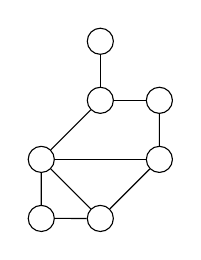
\begin{tikzpicture}[scale=0.75]
        \node [circle,draw] (1) at (0,0) {};
        \node [circle,draw] (2) at (0,-1) {};
        \node [circle,draw] (3) at (1,-1) {};
        \node [circle,draw] (4) at (-1,-2) {};
        \node [circle,draw] (5) at (1,-2) {};
        \node [circle,draw] (6) at (-1,-3) {};
        \node [circle,draw] (7) at (0,-3) {};
        
        \draw (1) -- (2);
        \draw (2) -- (3);
        \draw (3) -- (5);
        \draw (5) -- (7);
        \draw (7) -- (6);
        \draw (6) -- (4);
        \draw (4) -- (2);
        \draw (4) -- (7);
        \draw (4) -- (5);
    \end{tikzpicture}} \hspace{2cm}
    \subfloat[Not a tree - not connected  \label{fig:1b}]{
        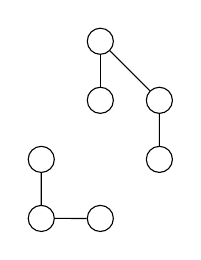
\begin{tikzpicture}[scale=0.75]
        \node [circle,draw] (1) at (0,0) {};
        \node [circle,draw] (2) at (0,-1) {};
        \node [circle,draw] (3) at (1,-1) {};
        \node [circle,draw] (4) at (-1,-2) {};
        \node [circle,draw] (5) at (1,-2) {};
        \node [circle,draw] (6) at (-1,-3) {};
        \node [circle,draw] (7) at (0,-3) {};
        
        \draw (1) -- (2);
        \draw (1) -- (3);
        \draw (3) -- (5);
        \draw (7) -- (6);
        \draw (6) -- (4);
    \end{tikzpicture}} \hspace{2cm}
\subfloat[A tree \label{fig:1c}]{
        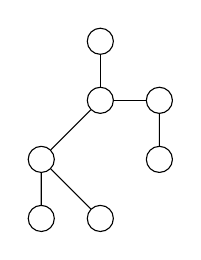
\begin{tikzpicture}[scale=0.75]
        \node [circle,draw] (1) at (0,0) {};
        \node [circle,draw] (2) at (0,-1) {};
        \node [circle,draw] (3) at (1,-1) {};
        \node [circle,draw] (4) at (-1,-2) {};
        \node [circle,draw] (5) at (1,-2) {};
        \node [circle,draw] (6) at (-1,-3) {};
        \node [circle,draw] (7) at (0,-3) {};
        
        \draw (1) -- (2);
        \draw (2) -- (3);
        \draw (3) -- (5);
        \draw (7) -- (4);
        \draw (6) -- (4);
        \draw (4) -- (2);
    \end{tikzpicture}} 
    \caption{Examples of graphs.}
\end{figure}

\end{exa}

    A \emph{subgraph} of a graph $G = (V,E)$ is a graph $G' = (V',E')$ with $V' \subseteq V$ and $E \subseteq E'$. If for every pair of vertices $v_1,v_2 \in G$ we have that $G'$ satisfies \[\{v_1,v_2\} \in E \text{ and } v_1,v_2 \in V' \implies \{v_1,v_2\} \in E',\] 
    then we say that $G'$ is the \emph{induced subgraph} of $G$ over $V'$. When $G$ is a tree, we typically use the terms \emph{subtree} and \emph{induced subtree} instead of subgraph and induced subgraph, respectively.


    A vertex of a tree is called a \emph{leaf node} if it is incident to exactly one edge. Otherwise, it is called a \emph{branch node}. It can be useful to distinguish a single node of a tree $T$ as a \emph{root node}, which we denote $R = \Root(T)$. A tree with a root is called \emph{rooted tree}. A rooted tree imposes a partial order $\prec$ on the vertices of a tree, where 
    \[ v_1 \prec v_2 \iff \dist(R, v_1) + \dist(v_1, v_2) = \dist(R, v_2).\] 
    (The Hasse diagram for this partial order on a tree is the tree itself!) If $v_2 \succ v_1$ and $v_2 \neq v_1$, $v_2$ is a \emph{descendant} of $v_1$. Each of the adjacent vertices to $R$ are \emph{children} of the root.


\begin{defin}
     Let $T$ be a rooted tree, and let $\{v_1, \ldots, v_n\}$ be the nodes adjacent to $\Root(T)$. A \emph{descendant subtree} of $T$ is a rooted, induced subtree of $T$ over the set containing vertex $v_i$ and its descendants with $v_i$ as its root. Since this is the only kind of subtree we discuss in the rest of these appendices, we refer to descendant subtrees as subtrees for simplicity. 
\end{defin}

Note that this definition requires us to impose some order on the children of each node in a rooted tree.

\begin{exa}
If we distinguish the node labeled 1 as the root in Figure 2,

\begin{figure}[H]
  \centering
    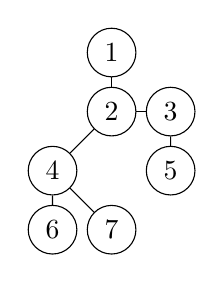
\begin{tikzpicture}[scale=0.75]
        \node [circle,draw] (1) at (0,0) {1};
        \node [circle,draw] (2) at (0,-1) {2};
        \node [circle,draw] (3) at (1,-1) {3};
        \node [circle,draw] (4) at (-1,-2) {4};
        \node [circle,draw] (5) at (1,-2) {5};
        \node [circle,draw] (6) at (-1,-3) {6};
        \node [circle,draw] (7) at (0,-3) {7};
        
        \draw (1) -- (2);
        \draw (2) -- (3);
        \draw (3) -- (5);
        \draw (7) -- (4);
        \draw (6) -- (4);
        \draw (4) -- (2);
    \end{tikzpicture}
    \caption{A labeled tree.}
\end{figure}

the graph corresponding to the figure has only one subtree, shown in Figure 3. The roots of each tree are shown in red.

\begin{figure}[H]
  \centering
    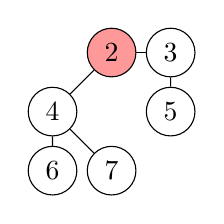
\begin{tikzpicture}[scale=0.75]
        \node [circle,draw, fill=red!40] (2) at (0,-1) {2};
        \node [circle,draw] (3) at (1,-1) {3};
        \node [circle,draw] (4) at (-1,-2) {4};
        \node [circle,draw] (5) at (1,-2) {5};
        \node [circle,draw] (6) at (-1,-3) {6};
        \node [circle,draw] (7) at (0,-3) {7};
        
        \draw (2) -- (3);
        \draw (3) -- (5);
        \draw (7) -- (4);
        \draw (6) -- (4);
        \draw (4) -- (2);
    \end{tikzpicture}
    \caption{Subtree of Figure 2 with 1 as the root.}
\end{figure}

If instead, the node labeled 2 is chosen as the root, the tree has three subtrees, shown in Figure 4.

\begin{figure}[H]
  \centering
    \subfloat[]{
    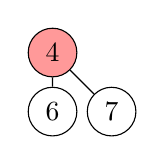
\begin{tikzpicture}[scale=0.75]
        \node [circle,draw, fill=red!40] (4) at (-1,-2) {4};
        \node [circle,draw] (6) at (-1,-3) {6};
        \node [circle,draw] (7) at (0,-3) {7};
        
        \draw (4) -- (6);
        \draw (4) -- (7);
    \end{tikzpicture}} \hspace{2cm}
    \subfloat[]{
        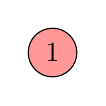
\begin{tikzpicture}[scale=0.75]
        \node [circle,draw, fill=red!40] (1) at (0,0) {1};
    \end{tikzpicture}} \hspace{2cm}
\subfloat[]{
        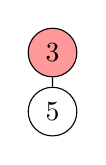
\begin{tikzpicture}[scale=0.75]
        \node [circle,draw, fill=red!40] (3) at (1,-1) {3};
        \node [circle,draw] (5) at (1,-2) {5};
        
        \draw (3) -- (5);
    \end{tikzpicture}} 
    \caption{Subtrees of Figure 2 with 2 as the root.}
\end{figure}

Subtree (a) has the node labeled 4 as its root, subtree (b) has 1, and subtree (c) has 3.

\end{exa}

\begin{defin}
    We \emph{construct} a new rooted tree $T' = (V', E')$ from rooted trees $T_1 = (V_1, E_1), \ldots ,T_n = (V_n, E_n)$, where every pair of vertex sets is disjoint, and a brand new node $v$ where $v \notin V_i$ for $i \in \{1, \ldots, n\}$ as follows:
    
    \begin{equation*}
        \construct(v, (T_1, \ldots T_n)) = T' = (V', E'),
    \end{equation*}
    
    where
    \begin{align*}
        V' &= \bigcup\limits_{i=1}^{n}V_i \cup\{v\},\\
        E' &= \bigcup\limits_{i=1}^{n}(E_i \cup \{v, \Root(T_i)\}), \text{ and }\\
        \Root(T') &= v.
    \end{align*}
\end{defin}

The operations $\subtree$ and $\construct$ are, in some sense, inverses, since if $T$ is a rooted tree with $\Root(T)$ adjacent to $n$ other vertices, 

\begin{equation*}
    \construct(\Root(T), \{\subtree(T,1), \ldots, \subtree(T, n)\}) = T.
\end{equation*}

We can use trees to represent the structure of expressions by anchoring the node with the outermost operation as the root node of the tree, with each of its children as operands. Each of those children's children are then operands to that child, and so forth.

Expressions can, of course, contain multiple of the same symbol, but every element of a set is unique. To allow multiple instances of a symbol in the vertex set, we index each vertex with a unique natural number.

\begin{defin} \label{def2}
    An \emph{expression tree} is a rooted tree $T = (V, E) \in \mathcal{X}(S, A, F)$ that satisfies the following:
    \begin{itemize}
        \item If $|V| = 1$, then the single vertex $v \in V$ must have $v = (v', i)$ for some $v' \in S \cup A, i \in \mathbb{N}$.
        \item If $|V| > 1$, then any leaf node $v \in V$ that is not the root node must have $v = (v', i)$ for some $v' \in S \cup A, i \in \mathbb{N}$. Every other node must have $v = (v', i)$ for some $v' \in F, i \in \mathbb{N}$.
        \item If $v \in V$ and $v = (f, i)$, for some $f \in F$ with $f$ having $n$ inputs, then $v$ must be incident with exactly $n+1$ edges.
    \end{itemize}
\end{defin}

To reduce the notational burden, $v = (v', i) \in V$ is represented as $v'$, so we can write $v \in S$, $v \in A$, or $v \in F$ as shorthand, for instance. Furthermore, we represent a tree with one vertex as the vertex itself, so we can say $T \in S$ or $T \in A$ if $\Root(T) \in S$ or $\Root(T) \in A$. See Example \ref{exa1} and Example \ref{exa2} for an extended example of how these trees are represented.

\begin{exa}
    Using the set $\mathcal{X}(S, A, F)$ from Example \ref{exa0}, we also write the symbol, constant, or function in a circle in the diagram of an expression tree to represent the element of $S$, $A$, or $F$ present at the vertex. Rather than coloring the root, from now on we use the convention that the root of the tree is the topmost node in the diagram.
    \begin{figure}[H]
  \centering
    \subfloat[Not an expression tree - does not satisfy the third part of definition \ref{def2}. \label{fig:2a}]{
            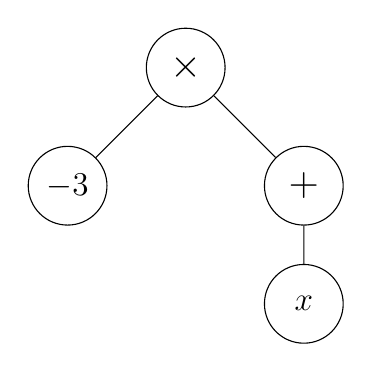
\begin{tikzpicture}[scale=0.75]
            \node [circle,draw,minimum width=1cm] (1) at (0,0) {\Large $\times$};
            \node [circle,draw,minimum width=1cm] (2) at (2,-2) {\Large $+$};
            \node [circle,draw,minimum width=1cm] (3) at (-2,-2) {\large $-3$};
            \node [circle,draw,minimum width=1cm] (4) at (2,-4) {\large $x$};
            
            \draw (1) -- (2);
            \draw (1) -- (3);
            \draw (2) -- (4);
        \end{tikzpicture}} \hspace{2cm}
    \subfloat[An expression tree - corresponding to $-3 \times (x + 1)$ \label{fig:2b}]{
        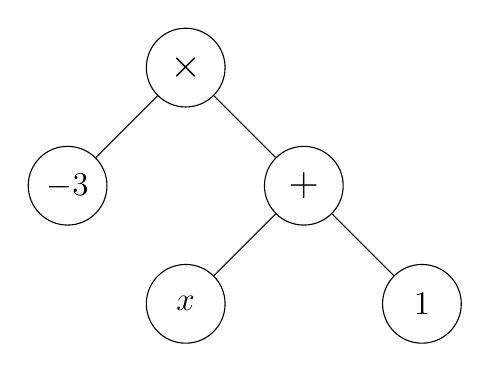
\begin{tikzpicture}[scale=0.75]
        \node [circle,draw,minimum width=1cm] (1) at (0,0) {\Large $\times$};
        \node [circle,draw,minimum width=1cm] (2) at (2,-2) {\Large $+$};
        \node [circle,draw,minimum width=1cm] (3) at (-2,-2) {\large $-3$};
        \node [circle,draw,minimum width=1cm] (4) at (0,-4) {\large $x$};
        \node [circle,draw,minimum width=1cm] (5) at (4,-4) {\large $1$};
        
        \draw (1) -- (2);
        \draw (1) -- (3);
        \draw (2) -- (4);
        \draw (2) -- (5);
    \end{tikzpicture}}
    \caption{Graphs and Expression Graphs}
\end{figure}
\end{exa}

\begin{defin}
    Expressions consisting of a single symbol or constant (so the corresponding expression tree has $|V| = 1$) are \emph{atomic expressions}, since they cannot be divided into \emph{subexpressions}, which are just subtrees of an expression tree. All other expressions are \emph{compound expressions}, consisting of one or more subexpressions. Also, if $X \in \mathcal{X}(S,A,F)$ is an expression, we let the function $\args(X)$ denote the number of subexpressions of $X$.
\end{defin}

\subsection{Ring Expressions}

While expression trees are versatile enough to represent structures of predicates from logic, sets from mathematics and vectors and matrices from linear algebra, the core functionality of a CAS is, unsurprisingly, algebra. The algebra of ring theory is a common choice, since it has a variety of operations to use without being too restrictive as to what constants we have available. Common algebraic structures such as integers, rational numbers, and polynomials are all rings, which is another bonus.

\begin{defin}
    A \emph{ring} is a 3-tuple $(R, +, \times)$, where $R$ is a set, and $+$, $\times$, are functions from $R^2 \to R$ that satisfy the following properties:
    
    \begin{description}[style=multiline,
            topsep=5pt,
            leftmargin=5.5cm]
        \item[\emph{Additive associativity:}] $\forall x, y \in R$, $((x + y) + z) = (x + (y + z))$
        \item[\emph{Additive identity:}] $\exists 0 \in R$ such that $\forall x \in R$, $x+0=0+x=0$
        \item[\emph{Additive inverse:}] $\forall x \in R$, $\exists y \in R$ such that $x + y = y + x = 0$
        \item[\emph{Additive commutativity:}] $\forall x, y \in R$, $x + y = y + x$
        \item[\emph{Multiplicative associativity:}] $\forall x, y \in R$, $((x \times y) \times z) = (x \times (y \times z))$
        \item[\emph{Multiplicative identity:}] $\exists 1 \in R$ such that $\forall x \in R$, $x\times 1 = 1 \times x=1$
        
        \item[\emph{Distributive Property:}] $\forall x,y,z \in R$, $x \times (y + z) = x\times y + x\times z$ and $(y + z) \times x = y\times x + y\times x$
    \end{description}
\end{defin}

Multiplication of two ring elements $x \times y$ is usually written as $xy$. For an in-depth introduction to ring theory and the theory of other algebraic structures, see \cite{aa}.

A ring $R$ is a \emph{commutative ring} if it satisfies
\begin{equation*}
        \forall x,y \in R, x \times y = y \times x.
\end{equation*}

The commutativity of multiplication is not assumed in a general ring, but most common rings, including all rings in the algebra package, have this property.

An \emph{integral domain} is a commutative ring $R$ if it further satisfies

\begin{equation*}
        \forall x,y \in R, x \neq 0 \text{ and } y \neq 0 \implies xy \neq 0.
\end{equation*}

Rings such as the integers are also Euclidean domains, which ensure the division with remainder and modulo operations are easily understood. Formally, $R$ is a \emph{Euclidean domain} if $R$ is an integral domain and there is some function $f: R \to \mathbb{N}$ that satisfies
\begin{equation*}
    \forall a, b \in R, \exists q,r \in R \text{ such that } a = bq + r \text{ with } r = 0 \text{ or } f(r) < f(b).  
\end{equation*}

Finally, rings such as the rationals have multiplicative inverses for every element except $0$. When combined with commutativity, this makes the standard division operation well-defined. Formally, $R$ is a \emph{field} if it is commutative and

\[ \forall x \in R, \text{ if } x \neq 0, \text{ then } \exists y \in R \text{ such that } xy=yx=1.\] 

All rings also have an exponentiation operation that can be defined analogous to exponentiation as is commonly used. Exponentiation is a function from $R \times \mathbb{N}$ to $R$, and is denoted as $x \pow n$ or $x^n$ for $x \in R$, $n \in \mathbb{N}$. Exponentiation is defined as follows:

\begin{equation*}
    x^n = \begin{cases} 1 & n = 0\\
                (x)(x^{n-1}) & n > 0.
                \end{cases}
\end{equation*}

If $R$ is also a field, the exponent domain can be extended to $\mathbb{Z}$ as follows, assuming $x$ is not the zero element of the field and $y$ is the multiplicative inverse of $x$:

\begin{equation*}
    x^n = \begin{cases} 1 & n = 0\\
                (x)(x^{n-1}) & n > 0\\
                y^{-n} & n < 0.
                \end{cases}
\end{equation*}

The following example illustrates how expression trees are constructed for the field of rational numbers. By the end of the example, it will be a close analog of the actual implementation of expression trees in the CAS.

\begin{exa} \label{exa1}
    Let $S = \{a, b, c, \ldots, x, y, z, A, B, C, \ldots, X, Y, Z, \_\}^+$, $A = \mathbb{Q}$, and $F = \{+, - , \times, /, \pow\}$ as in Definition \ref{def1}. The operations $+$, $\times$, and $\pow$ are defined as usual for the field of rationals. The operations $-$ and $/$ are defined by taking the inverse of the second element of the first two operations: $x - y = x + (-y)$; $x / y = (x)(1/y)$.
    
    Unfortunately, this is not a proper expression tree yet. Some operators are not defined over all rational numbers - in particular, division is undefined when the second operand is zero, and exponentiation is undefined when the second operand is not an integer. 
    
    Most computer algebra systems, including this one (eventually!), fix this by outputting a special `not a number' constant $\NaN$, so $A$ can be changed to $\mathbb{Q} \cup \{\NaN\}$. Then, we extend the input of each operator by outputing $\NaN$ if any of the inputs are $\NaN$:
    
    \begin{equation*}
        \forall f \in F, f(\ldots,\NaN,\ldots) = \NaN
    \end{equation*}
    
    This behavior holds for all of the functions we will add in $F$. There are more notational quirks of the typical way algebraic expressions are written that we need to consider. Since addition and multiplication are associative, for instance $(x+y)+z = x+(y+z)$, we write either expression as $x+y+z$ without ambiguity. Associative operations almost always have parentheses omitted when writing, so
    
    \begin{equation*}
        x + (y + 1/5)
    \end{equation*}
    
    would be written
    
    \begin{equation*}
        x + y + 1/5.
    \end{equation*}
    
    We can account for this notation mathematically by replacing $+$ and $\times$ with their $n$-operand equivalents in $F$. Zero-operand addition and multiplication return $0$ and $1$ respectively, while single-operand addition and multiplication are identity functions.
    
    \begin{figure}[H]
    \centering
    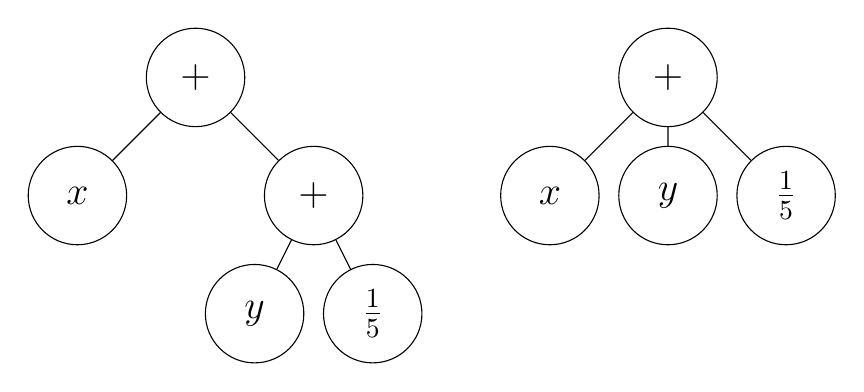
\begin{tikzpicture}[scale=0.75]
        \node [circle,draw,minimum width=1.25cm] (plus) at (0,0) {\Large $+$};
        \node [circle,draw,minimum width=1.25cm] (x) at (-2, -2) {\Large $x$};
        \node [circle,draw,minimum width=1.25cm] (plus2) at (2,-2) {\Large $+$};
        \node [circle,draw,minimum width=1.25cm] (y) at (1, -4) {\Large $y$};
        \node [circle,draw,minimum width=1.25cm] (1/3) at (3, -4) {\Large $\frac{1}{5}$};
        
        \node [circle,draw,minimum width=1.25cm] (plus3) at (8,0) {\Large $+$};
        \node [circle,draw,minimum width=1.25cm] (x2) at (6, -2) {\Large $x$};
        \node [circle,draw,minimum width=1.25cm] (y2) at (8, -2) {\Large $y$};
        \node [circle,draw,minimum width=1.25cm] (1/32) at (10, -2) {\Large $\frac{1}{5}$};
        
        
        \draw (plus) -- (x);
        \draw (plus) -- (plus2);
        \draw (plus2) -- (y);
        \draw (plus2) -- (1/3);
        
        \draw (plus3) -- (x2);
        \draw (plus3) -- (y2);
        \draw (plus3) -- (1/32);
    \end{tikzpicture}
    \caption{Example expression trees corresponding to $x + (y + 1/3)$ and $x + y + 1/3$. \label{fig:1}}
    \end{figure}
    
    Finally, the exponentiation operation is typically not thought of as undefined for non-natural powers -- consider $2^{1/2} = \sqrt{2}$, for instance. The result just happens to be outside the set of rationals. Rather than augmenting $A$ again, it would be cleaner to amend our expression definition so the domain and codomain of operations in $F$ include expression trees. 
\end{exa}

\begin{defin}
    (Revised) An \emph{expression} $X$ is a an element of the set $\mathcal{T} = \mathcal{X}(S,A,F)$, such that
    \begin{itemize}
                \item $S$ is a set of symbols,
    \item $A$ is a set of constants with $A \cap S = \emptyset$ and $\NaN \in A$, and
    \item $F$ is a set of operations with each $f \in F$ having $f: \mathcal{T}^n \to \mathcal{T}$ for some $n \in \mathbb{N}$.
    \end{itemize}
\end{defin}

This definition is more versatile, and allows us to define more complex operators like the derivative as being a part of an expression rather than just an operation on expressions, but it introduces the additional complexity of recursion.

\begin{exa} \label{exa2}
    Continuing from Example \ref{exa1}, we can leave the sets $S$ and $A$ alone for the revised definition, but functions $f$ now need to be extended to work for all expressions. For $+$, for instance, we let $x + y$ be defined as before if $x,y \in A$, and $\construct(+, (x,y))$ otherwise. Other operations work much the same, and $+$ and $\times$ use an $n$-tuple in the second argument to $\construct$ instead of a 2-tuple if there are $n$ arguments.
    
    One exception is exponentiation, where
    
    \begin{equation*}
        x \pow y = \begin{cases} x^y & x \in A, y \in \mathbb{Z}\\
                    \construct(\pow, (x,y)) & \text{otherwise}.
                    \end{cases}
    \end{equation*}
    

Trigonometric functions, logarithms, and any other special functions we desire can also be included in $F$. We also add the derivative to $F$ which takes two arguments, the first of which is an expression $X$ and the second of which is a variable $s \in S$. Rather than having to define limits over expression trees, we use a \emph{differential algebra} to define our derivative operator over $\mathcal{X}(S,A,F)$. For a complete description of a differential algebra, see Definition \ref{def8}. The differential algebra we use is the \emph{formal derivative}, which uses the standard properties of a differential algebra with the additional rule that $\frac{\mathrm{d}}{\mathrm{d}x}(x)=1$ for any variable $x \in S$.


We can represent the expression $\frac{\mathrm{d}}{\mathrm{d}x} (\sin (x) + 3x+6)$, for instance, as below:


\begin{figure}[H]
\centering
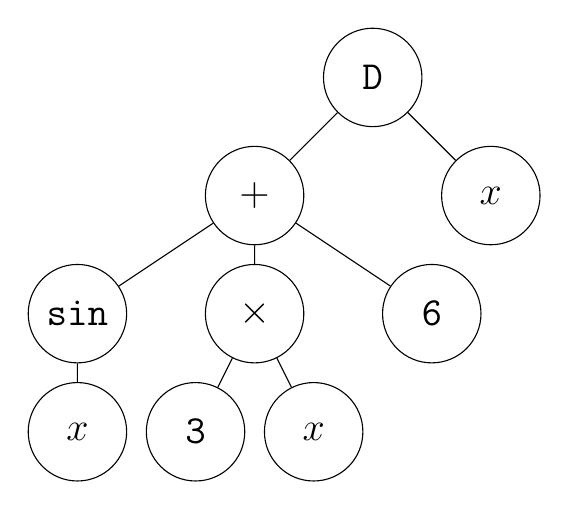
\begin{tikzpicture}[scale=0.75]
    \node [circle,draw,minimum width=1.25cm] (D) at (0,0) {\Large \ttfamily D};
    \node [circle,draw,minimum width=1.25cm] (plus) at (-2,-2) {\Large $+$};
    \node [circle,draw,minimum width=1.25cm] (x) at (2, -2) {\Large $x$};
    \node [circle,draw,minimum width=1.25cm] (sin) at (-5, -4) {\Large \ttfamily sin};
    \node [circle,draw,minimum width=1.25cm] (times) at (-2, -4) {\Large $\times$};
    \node [circle,draw,minimum width=1.25cm] (6) at (1, -4) {\Large \ttfamily 6};
    \node [circle,draw,minimum width=1.25cm] (x2) at (-5, -6) {\Large$x$};
    \node [circle,draw,minimum width=1.25cm] (3) at (-3, -6) {\Large \ttfamily 3};
    \node [circle,draw,minimum width=1.25cm] (x3) at (-1, -6) {\Large $x$};
    
    
    \draw (D) -- (plus);
    \draw (D) -- (x);
    \draw (plus) -- (sin);
    \draw (plus) -- (times);
    \draw (plus) -- (6);
    \draw (sin) -- (x2);
    \draw (times) -- (3);
    \draw (times) -- (x3);
\end{tikzpicture}
\caption{Example expression tree corresponding to $\frac{\mathrm{d}}{\mathrm{d}x}(\sin(x) + 3x + 6)$. \label{fig:2}}
\end{figure}

This expression tree illustrates a case where subtree order matters, since $\sin(x)+3x+6$ can only be the first subtree of the derivative.
    
    
\end{exa}

\subsection{Generic Expression Operations}

\begin{defin}
    \emph{Structural equality} $(=)$ is equality on a set of expression trees $\mathcal{X}(S, A, F)$ defined in the usual way using set and tuple equality, including the underlying equalities on $S$ and $A$.
\end{defin}

While structural equality is useful, it does not align with the conventional notion of equality that a user of our CAS would want. It will not return the expressions $x + x$ and $2x$, or even $(x + x) + x$ and $x + x + x$ as equal. For this, we need to define various operations that act on trees. (These could even be added as part of the $F$ set, if the expression structure is defined properly.)

\begin{defin}
    \emph{Evaluation} is a function that outputs the result of applying each function in a tree to its sub-tree recursively. Given an expression $X \in \mathcal{X} = \mathcal{X}(S, A, F)$,
    
    \begin{equation*}
        \eval(X) = \begin{cases}
                X & X \in S \cup A \\
                f(\eval(\subtree(X,1)), \ldots, \\ \eval(\subtree(X,m))) & \Root(X) = f \in F, f:\mathcal{X}^m\to\mathcal{X}
                \end{cases}
    \end{equation*}
    
    If $\eval(X) \in A$, then $X$ is \emph{evaluatable}. If $\eval(X) = X$, then $X$ is an \emph{evaluated expression}. 
\end{defin}


If for all $X \in \mathcal{X} = \mathcal{X}(S, A, F)$, there exists some natural number $n$ for which \[\eval^{n+1}(X) = \eval^n(X),\] then $\mathcal{X}$ is \emph{terminating}.
    
Evaluation is not a very useful procedure in actual CASs, but it is an important theoretical tool. To reduce the number of cases we need to consider in our algorithms, the set of evaluated expressions is typically the full subset of expressions we consider manipulating. This subset can further be reduced to autosimplified expressions (see Appendix B).

\begin{exa} Continuing from Example \ref{exa2}, expressions are evaluatable if and only if they do not contain symbols. For example,

\begin{align*}
    \eval(((3 - 4)x) - y) &= \eval((3-4)x)-\eval(y)\\
                        &= \eval(3-4)\eval(x) - y \\
                        &= (\eval(3)-\eval(4))x-y\\
                        &= (-1)(x)-y.
\end{align*}

Here, the subexpression $(3-4)$ is evaluatable, but the whole expression is not. Also, $\mathcal{X}(S, A, F)$ is a terminating set of expressions. In fact,

\begin{thm}
    Let $\mathcal{X}(S, A, F)$ be defined as in Example \ref{exa2}, except $F$ does not contain the derivative operator. Then, 
    
    \begin{equation*}
            \forall X \in \mathcal{X}, \eval(\eval(X)) = \eval(X).
    \end{equation*}

\end{thm}
\begin{proof}
    Proof by structural induction. Let $X \in \mathcal{X}$. If $X \in S \cup A$, then $\eval(X) = X$, so $\eval(\eval(X)) = \eval(X)$.
    
    Otherwise, assume each subtree of the $n$ subtrees of $X_i = \subtree(X, i)$ of $X$ has \[\eval(\eval(X_i)) = \eval(X_i).\] Let $f = \Root(X)$. If all subtrees have $X_i \in A$ (or $X_i \in \mathbb{N}$ if $f = \pow$), then $\eval(X) \in A$, so $\eval(\eval(X)) = \eval(X)$. Otherwise, every $f \in F$ has
    \begin{equation*}
            f(X_1, \ldots ,X_n) = \construct(f, (X_1, \ldots, X_n)) = X,
    \end{equation*}
    so again, $\eval(\eval(X)) = \eval(X)$.
\end{proof}

If the derivative operator is included in $F$, it is still true that $\mathcal{X}$ is terminating, since it can be shown that $\eval^3(X) = \eval^2(X)$ for every $X \in \mathcal{X}$.
    
\end{exa}

\begin{defin} \label{def3}
    \emph{Substitution} is a function that replaces variables in an expression with other expressions. Given an expression $X \in \mathcal{X} = \mathcal{X}(S, A, F)$, and a set of tuples $\mathcal{S} = \{(s_1, X_1), \ldots , (s_n, X_n)\}$, where each $s_i$ is a unique element of $S$ and each $X_i \in \mathcal{X}$,
    
    \begin{equation*}
        \subs(X, \mathcal{S}) = \begin{cases} 
                                  X & X \in A \\
                                  X &  X \in S \text{ and } X \neq s_i \forall i \\
                                  X_i & X \in S \text{ and } X = s_i\\
                                  f(\subs(\subtree(X, 1)),\ldots, \\ \subs(\subtree(X, m))) & \Root(X) = f \in F, f:\mathcal{X}^m\to\mathcal{X}
                               \end{cases}
    \end{equation*}
\end{defin} 

Substitution is an important procedure in CASs in its own right. It is used when evaluating polynomials, for instance. Note also the relation to evaluation - in fact, $\subs(X, \emptyset) = \eval(X)$.

\begin{exa}
    Continuing from Example \ref{exa2}, If $\mathcal{S} = \{(x, -2), (y, 2*y), (z, 4)\}$,
    
    \begin{align*}
            \subs(((3 - 4)x) - y, \mathcal{S}) &= \subs((3-4)x, \mathcal{S})-\subs(y, \mathcal{S})\\
                        &= \subs(3-4, \mathcal{S})\subs(x, \mathcal{S}) - 2y \\
                        &= (\subs(3, \mathcal{S})-\subs(4, \mathcal{S}))(-2)-2y\\
                        &= (-1)(-2)-2y\\
                        &= 2-2y.
    \end{align*}
\end{exa}

\begin{defin}  \label{def4}
    Two expressions $X_1, X_2$ in a terminating set of expressions $\mathcal{X}(S, A, F)$ are \emph{semantically equal}, $X_1\overset{s}{=}X_2$, if, for all $\mathcal{S} \in \mathcal{P}(S \times A)$ with $|\mathcal{S}| = |S|$ and the set of all first elements of the tuples of $\mathcal{S}$ equal to $S$,
    
    \begin{equation*}
        \subs(\eval^n(X_1), \mathcal{S}) = \subs(\eval^m(X_2), \mathcal{S})
    \end{equation*}
    
    where $n$ and $m$ are natural numbers such that $\eval^{n+1}(X_1) = \eval^n(X_1)$ and $\eval^{m+1}(X_2) = \eval^m(X_2)$.
\end{defin}

This definition is not defined by any structure on the underlying set $A$, but instead by the notion that every possible substitution of variables in $S$ for two expressions results in the same element of $A$.

The termination requirement is due to the fact that both expressions must be evaluated expressions to ensure operations that act on trees and are part of $F$, such as the derivative, are semantically equal to their evaluations, so, for instance,

\begin{equation*}
    \frac{\mathrm{d}}{\mathrm{d}x} (x^2) \overset{s}{=} x+x 
\end{equation*}

would not work if the evaluation functions where not included.

Sets of operations that result in expression sets that are not terminating are somewhat contrived anyway. The most obvious example are including functions in $F$ that return a modified version of themselves:

\begin{equation*}
    f(X) = \construct(+, (f(X), 1))
\end{equation*}

Semantic equality in the usual sense is ill-defined for these expressions anyway, since it would seem that

\begin{equation*}
    f(X) \overset{s}{=} f(X) + 1 \overset{s}{=} (f(X) + 1)  + 1\overset{s}{=} \ldots
\end{equation*}

\begin{thm}
    If $\mathcal{X}(S,A,F)$ is a terminating set of expressions, $\overset{s}{=}$ is an equivalence relation on $\mathcal{X}(S,A,F)$.
\end{thm}

The proof largely follows from the fact that structural equality is an equivalence relationship on $\mathcal{X}(S,A,F)$ The details are left to the reader.

\subsection{Implementation Details}

While mathematically rigorous definitions of expression trees can be rather cumbersome, they are natural to implement as data structures in code. In Lua, this means using tables. Lua does not have built-in object-oriented functionality like Python or Java - instead, we use prototypes. \cite{pil} A prototype is a single table that acts like a class. It has a {\ttfamily new} method that can be used to construct tables, which correspond with objects. These objects have specific functions and variables as entries, which correspond to methods and instance variables, respectively. This is further streamlined by creating a metatable for the object and setting the {\ttfamily \_\_index} field to the class itself. The {\ttfamily \_\_index} field's entries, which are the class's entries, are accessed if no entry is found in the table the metatable is assigned to. Example code for creating an object in the ring of rationals is shown below:

\inputminted[
firstline=13,
lastline=52,
breaklines]
{lua}
{algebra/rational.lua}

Inheritance can also be implemented in Lua using the {\ttfamily \_\_index} metamethod, since it works recursively. If a class has an {\ttfamily \_\_index} metamethod then it can call methods from its superclass. The exception to this is other metamethods, which must be set in the metatable of the object itself. Interface implementation isn't necessary in Lua due to weak typing, but can still be implemented in spirit by adding superclasses with methods that throw errors for any methods that a subclass must implement.

Creating the prototypes for expression trees is as simple as creating a prototype for a general expression, and two prototypes for atomic and compound expressions that inherit their properties from general expressions. Compound expressions have one or more general expressions as instance variables, thus completing the recursive tree structure.

The various ring classes implemented in the algebra package - integers, integer mod rings, rationals, and polynomials - all inherit from atomic expressions. The various functions and operations, including binary operations ($+$, $\times$, $-$, $/$, and $\pow$), derivatives, integrals, and special functions all inherit from compound expressions. Each object created from a prototpye is an expression tree.

The code for substitution is split across different classes (compare with Definition \ref{def3}):

\inputminted[
firstline=44,
lastline=51,
breaklines]
{lua}
{core/atomicexpression.lua}

\inputminted[
firstline=23,
lastline=35,
breaklines]
{lua}
{core/compoundexpression.lua}


\newcommand{\iClass}{\tikz[baseline=-0.75ex]{\node[circle,draw,draw=violet!75!black,fill=violet!30,text=black,inner sep=1pt]{\bfseries\ttfamily I};}\,}

\newcommand{\cClass}{\tikz[baseline=-0.75ex]{\node[circle,draw,draw=red!75!black,fill=green!30,text=black,inner sep=1pt]{\bfseries\ttfamily C};}\,}

\tikzstyle{class}=[rectangle,
    draw=violet!75!black, 
    rounded corners=1pt, 
    fill=yellow!30, 
    drop shadow,
    align=left,
    text=black,
    font=\footnotesize\sffamily,
    rectangle split,
    rectangle split parts=3,
    rectangle split part align={left,left,left}]
    
\tikzstyle{inherit}=[-{Triangle[open,scale=1.5]},red!75!black]
\tikzstyle{has}=[-{Triangle[scale=1.5]},red!75!black]

\tikzset{package/.style args={#1}{
    draw,
    thick,
    inner sep=7pt,
    rectangle,
    rounded corners=1pt,
    label={[draw,trapezium,thick,outer sep=0pt,inner sep =2pt]\footnotesize\sffamily\bfseries #1}
    }
}

A simplified inheritance hierarchy is shown below:

\begin{figure}[H]
\centering
\begin{tikzpicture}[remember picture]
    \node [class] (cexpression)
        {\iClass\itshape CompoundExpression
        };
    
    \node[class,right=of cexpression] (expression)
        {\iClass\itshape Expression
        \nodepart{third} evaluate() \\
            substitute(map)\\
            autosimplify()
            
    };
    
    \node[class,right=of expression] (aexpression)
    {\iClass\itshape AtomicExpression
    };
    
    \node[class,below=of aexpression] (constant)
    {\raisebox{1.5ex}{\iClass}\itshape ConstantExpression
    };
    
    \node[class,left=of constant] (symbol)
    {\cClass\itshape SymbolExpression
        \nodepart{second} symbol
    };
    
    \node[class,left=of symbol] (function)
    {\cClass\itshape Function
    };
    
    \node[class,left=of function] (binop)
    {\cClass\itshape BinaryOp
        \nodepart{second} operation
        \nodepart{third}  isassociative()\\
                          iscommutative()
    };
    
    
    \node[class,below=1.5cm of constant] (ring)
    {\raisebox{1.5ex}{\iClass}\itshape Ring
        \nodepart{third} $+$ $-$ $\times$ \\
        zero() \\
        one()
    };
    
        \node[class,below=of ring] (euclid)
    {\raisebox{1.5ex}{\iClass}\itshape EuclideanDomain
        \nodepart{third} $\mod$
    };
    
    \node[class,below=of euclid] (field)
    {\raisebox{1.5ex}{\iClass}\itshape Field
        \nodepart{third} $\div$
    };
    
    \node[class, left=of ring] (polynomial)
    {\cClass\itshape PolynomialRing
    };
    
    \node[class, left=of euclid] (integer)
    {\cClass\itshape Integer
        \nodepart{two} digits[]
    };
    
    \node[class, left=of field] (rational)
    {\cClass\itshape Rational
    };
    
    \node[class, left=of integer] (mod)
    {\cClass\itshape IntegerModRing
    };
    
    
    
    \draw [inherit] (cexpression.one east) -- (expression.one west) ;
    \draw [inherit] (aexpression.one west) -- (expression.one east);
    \draw [has] (cexpression.two east) -- (expression.two west) node[below,midway] {0..*};
    \draw [inherit] (symbol.one north) -- (aexpression.three south);
    \draw [inherit] (constant.one north) -- (aexpression.three south);
    
    \draw [inherit] (binop.one north) --  (cexpression.three south);
    \draw [inherit]  (function.one north) -- (cexpression.three south);
    
    \draw [has] (function.two east) --
    (symbol.one west) node[above,midway] {1};
    
    
    \draw [inherit] (ring.one north) -- (constant.three south);
    
    \draw [inherit] (euclid.one north) --(ring.three south);
    
    \draw [inherit] (field.one north) -- (euclid.three south);
    
    \draw [inherit] (polynomial.one east) -- (ring.one west);
    
    \draw [inherit] (integer.one east) -- (euclid.one west);
    
    \draw [inherit] (rational.one east) -- (field.one west);
    
    \draw [inherit] (mod.one east) -- (ring.three west);
    
    \draw [has] (mod.two east) -- (integer.one west) node[above,midway] {2};
    \draw [has] (rational.one north) -- (integer.three south) node[above,midway] {2};
    
    \draw [has] (polynomial.two east) -- (ring.two west) node[above,midway] {1..*};
    \draw [has] (polynomial.one north) -- (symbol.three south) node[below left] {1};
    
    \node[package={Core},
    fit=(cexpression)(expression)(aexpression)(constant)(symbol)(binop)(function)] (exp) {};
    
    \node[package={Algebra},
    fit=(ring)(euclid)(field)(polynomial)(rational)(integer)(mod)] (exp) {};
    
\end{tikzpicture}
\caption{Simplified UML class diagram for expressions and the algebra package.}
\end{figure}

Note here the parallels between the mathematical and class structures: All fields are euclidean domains, which in turn are rings. Objects are thus elements of the structure (class) they are instantiated from. Polynomial rings are dynamically created as either rings or euclidean domains depending on whether the underlying ring is a field or not. Similarly, Integer Mod Rings are instantiated as fields if the modulus used to create them is prime. The seeming lack of respect for software engineering principles here is in part due to the nature of building a computer algebra system itself (a field is always going to be a ring, so we don't need to favor composition over inheritance) and partly due to the peculiar nature of OOP in Lua. (Just try doing conditional inheritance in Java!)

\newpage

\section{Autosimplification}

\textit{Simplification}, broadly speaking, is the conversion of expressions into other expressions that are less complicated or easier to read. \textit{Automatic simplification}, or \textit{autosimplification}, is a simplification algorithm done on all expressions input into the CAS and output to the user. \cite{casc2} An expression that is the output of an autosimplification algorithm is called an \textit{autosimplified expression}. The primary purpose of autosimplification is to reduce the set of expressions we have to consider in most functions that act on expressions to just autosimplified expressions, as well as to display output to the user in a reasonable-looking way.

We can also have more theoretical aims, though. Definition \ref{def4} does not give a viable procedure for determining whether two expressions are semantically equal, since we would need to perform infinitely many substitutions if either the $S$ set or $A$ set is infinitely large. Using autosimplification, we might hope that we can reduce the problem of determining semantic equality to determining structural equality. Specifically, given an expression set $\mathcal{X} = \mathcal{X}(S,A,F)$, we would like

\begin{equation*}
    \forall X_1, X_2 \in \mathcal{X}, X_1 \overset{s}{=} X_2 \iff \Autosimplify(X_1) = \Autosimplify(X_2).
\end{equation*}

Unfortunately, this is not feasible to achieve. First, continuing with the expression set from the Appendix A examples, a user of our CAS would likely want

\begin{equation*}
    \Autosimplify\left(\frac{x}{x}\right) = 1,
\end{equation*}

however, $\frac{x}{x} \overset{s}{\neq} 1$, since $\subs(\frac{x}{x}, \{(x, 0)\}) = \NaN$, but $\subs(1, \{(x, 0)\}) = 1$. This particular scenario can be remedied by relaxing strict semantic equality slightly:

\begin{defin}
    Two expressions $X_1, X_2$ in a terminating set of expressions $\mathcal{X}(S, A, F)$ are \emph{definitely semantically equal}, $X_1\overset{s}{\approx}X_2$, if, for all $\mathcal{S} \in \mathcal{P}(S \times A)$ with $|\mathcal{S}| = |S|$ and the set of all first elements of the tuples of $\mathcal{S}$ equal to $S$,
    
    \begin{equation*}
        \subs(\eval^n(X_1), \mathcal{S}) = \subs(\eval^m(X_2), \mathcal{S}),
    \end{equation*}
    
    or
    
    \begin{equation*}
    \subs(\eval^n(X_1), \mathcal{S}) = \NaN, \text{ or } \subs(\eval^m(X_2), \mathcal{S}) = \NaN,
    \end{equation*}
    
    where $n$ and $m$ are natural numbers such that $\eval^{n+1}(X_1) = \eval^n(X_1)$ and $\eval^{m+1}(X_2) = \eval^m(X_2)$.
\end{defin}

Definite semantic equality, like semantic equality, is an equivalence relation on a terminating set of expressions. Furthermore, semantic equality implies definite semantic equality.

However, it is still infeasible to enforce

\begin{equation*}
    \forall X_1, X_2 \in \mathcal{X}, X_1 \overset{s}{\approx} X_2 \iff \Autosimplify(X_1) = \Autosimplify(X_2)
\end{equation*}

for the functionality of our computer algebra system. For instance, consider the expression $(x+1)^{1000}$. Expanding the expression using the binomial theorem gives \[(x+1)^{1000} \overset{s}{=} x^{1000}+\binom{1000}{1} x^{999}+ \ldots + \binom{1000}{999} x+1.\] Clearly, the expression $(x+1)^{1000}$ is `simpler' (if we wanted an exact notion of simplicity, we could use the number of vertices in corresponding expression trees). However, autosimplifying the later expression into the former requires factoring a 1000-degree polynomial, which is slow. Since autosimplify is called by our CAS for every entered expression, sometimes multiple times, it needs to be fast, which factoring a large polynomial is generally not (see Appendix C).

The most we could hope for, then, from an autosimplification procedure is:

\begin{equation*}
    \forall X_1, X_2 \in \mathcal{X}, \Autosimplify(X_1) = \Autosimplify(X_2) \implies X_1 \overset{s}{\approx} X_2. 
\end{equation*}


(This does not mean we shouldn't try to reduce as many semantically equal expressions to structurally equal expressions as is reasonable!) We would also like all autosimplified expressions to always autosimplify to themselves, so if the user takes output from the CAS and inputs it back in, the new output is always the same as the old output (Looking at you, Maple!):

\begin{equation*}
    \forall X \in \mathcal{X}, \Autosimplify(\Autosimplify(X)) = \Autosimplify(X).
\end{equation*}

\begin{defin} \label{def5}
    \emph{Autosimplification} is a function that transforms expressions into simpler expressions. The following procedure defines generic autosimplification: 
    
    \begin{algorithm}\small
    \caption{Generic Autosimplification Algorithm}
        \begin{algorithmic}[1]
            \Require $X \in \mathcal{X}(S, A, F)$
            \Ensure $X$ is autosimplified  
            \If{$X \in S \cup A$}
                \State \Return $X$
            \Else
                \For{$i \in \{1, \ldots, \args(X)\}$}
                    \State $X_i \gets \subtree(X, i)$
                    \State $X_i \gets \Autosimplify(X_i)$
                \EndFor
                \State $X \gets \construct(\Root(X), \{X_1, \ldots, X_{\args(X)}\})$
                \State \Return $\arules(X)$
            \EndIf
        \end{algorithmic}
    \end{algorithm}
\end{defin}

\emph{Autosimplification rules} are a set of transformations from expressions to expressions that depend on the set of functions in $F$, and may be complex functions themselves.

\begin{thm}
    If, for all $ X \in \mathcal{X}(S, A, F)$, $\arules(X) \overset{s}{\approx} X$, then $\forall X_1, X_2 \in \mathcal{X}(S, A, F)$, $\Autosimplify(X_1) = \Autosimplify(X_2) \implies X_1 \overset{s}{\approx} X_2$. 
\end{thm}

This theorem is straightforward, but it is useful because it allows us to use properties of the $S$ set to construct autosimplification rules.

Due to the autosimplification rules, the nature of autosimplification is heavily dependent on the structure underlying the set of expressions. Our discussion, then, is focused on the $\mathcal{X}(S, A, F)$ set developed in Example \ref{exa1}, as it mirrors the expression trees in the CAS. See Example \ref{exa3} for the autosimplification algorithm in practice.

\subsection{Autosimplification Over Fields}

Before we start defining our autosimplification rules, there is one caveat we need to address. The commutativity of multiplication and addition mean that we can rearrange $n$-ary sums and products in any order and still maintain semantic equality:

\begin{equation*}
    x+2y+3z^2 \overset{s}{=} 2y+3z^2+x \overset{s}{=} 3z^2+2y+x \overset{s}{=} \ldots
\end{equation*}

Thus, for the autosimplifications of these expressions to be structurally equal, we need to maintain a total order $\lhd$ on all autosimplified expressions, and our simplification rules need to sort the subexpressions of sum expressions and product expressions by $\lhd$.


\begin{defin}
    Let $\mathcal{X} = \mathcal{X}(S, A, F)$ be defined as in Example \ref{exa2}, and $\leq$ be the standard linear order on $\mathbb{Q}$ and the standard lexographic order on $A$. Let $\lhd$ be the binary relation on $\mathcal{X}$ defined by the Algorithm \ref{alg1}, which returns {\ttfamily true} if and only if $(U, V) \in \lhd$.
    
    
    \begin{algorithm}\small
    \caption{Total Order on Expressions $\lhd$} \label{alg1}
        \begin{algorithmic}[1]
            \Require $U, V \in \mathcal{X}(S, A, F)$ \AND $U, V$ autosimplified
            \State $m \gets \args(U)$, $n \gets \args(V)$
            \If{$U,V \in A$}
                \State \Return $U \leq V$
            \ElsIf{$U,V \in S$}
                \State \Return $U \leq V$
            \ElsIf{$\Root(U) = \Root(V) = +$ \OR $\Root(U) = \Root(V) = \times$ }
                \For{$i \in \{0, \ldots, \min\{m,n\} - 1\}$}
                    \If{$\subtree(U, m-i) \neq \subtree(U, n-i)$}
                        \State \Return $\subtree(U, m-i) \lhd \subtree(U, n-i)$
                    \EndIf
                \EndFor
                \State \Return $m \leq n$
            \ElsIf{$\Root(U) = \Root(V) = \pow$}
                \If{$\subtree(U, 1) \neq \subtree(V, 1)$}
                    \State \Return $\subtree(U, 1) \lhd \subtree(V, 1)$ 
                \Else 
                \State \Return $\subtree(U, 2) \lhd \subtree(V, 2)$
                \EndIf
            \ElsIf{$\Root(U)$ and $\Root(V)$ are both special functions}
                \If{The name of $\Root(U)$ precedes the name of $\Root(V)$ in $\leq$}
                    \State \Return $\Root(U)\leq \Root(V)$
                \Else
                    \For{$i \in \{1, \ldots, \min\{m,n\}\}$}
                        \If{$U_i \neq U_j$}
                            \State \Return $U_i \lhd U_j$
                        \EndIf
                    \EndFor
                    \State \Return $m \leq n$
                \EndIf
            \ElsIf{$U \in A$ \AND $V \not \in A$}
                \State \Return $U \lhd V$
            \ElsIf{$\Root(U) = \times$ \AND $V \not \in A$ \AND $\Root(V) \neq \times$}
                \State \Return $U \lhd \construct(\times, \{V\})$
            \ElsIf{$\Root(U) = \pow$ \AND $V \not \in A$ \AND $\Root(V) \neq \times$ \AND $\Root(V) \neq \pow$}
                \State \Return $U \lhd \construct(\times, \{V, 1\})$
            \ElsIf{$\Root(U) = +$ \AND $V \in S$ \OR $\Root(V)$ is a special function}
                \State \Return $U \lhd \construct(+, \{V\})$
            \ElsIf{$\Root(U)$ is a special function \AND $V \in S$}
                \State \Return $\Root(U) \leq \Root(V)$
            \Else
                \State \Return \NOT $v \lhd u$
            \EndIf
        \end{algorithmic}
    \end{algorithm}
\end{defin}


\begin{thm}
    The binary relation $\lhd$ is a total order on autosimplifed expressions in $\mathcal{X}$.
\end{thm}

The total order also effects the output of expressions in the CAS so that they are displayed naturally. Even if $y^23x$ and $3xy^2$ are semantically equal, the later looks more natural to our users.

\begin{exa}
    We determine the order of the expressions
    \begin{equation*}
       c(x+4y^2) \text{ and } (a+3b^2)(x+4y^2).
    \end{equation*}
    
    Each line of pseudocode used in the recursive computation of $\lhd$ is shown below.
    \begin{center}
    \begin{tabular}{|c|c|c|c|c|}
        \hline 
        $U$& $V$& $\Root(U)$ & $\Root(V)$ & Code \\
        \hline
         $c(x+4y^2)$& $(a+3b^2)(x+4y^2)$&$\times$&$\times$&\ref{alg1}.9, $i=1$\\
         $c$&$a+3b^2$&$c$&$+$&\ref{alg1}.41\\ 
         $a+3b^2$&$c$&$+$&$c$&\ref{alg1}.36\\
         $a+3b^2$&$+c$&$+$&$+$&\ref{alg1}.9, $i=0$\\
         $3b^2$&$c$&$\times$&$c$&\ref{alg1}.32\\
         $3b^2$&$\times c$&$\times$&$\times$&\ref{alg1}.9, $i=0$\\
         $b^2$&$c$&$\pow$&$c$&\ref{alg1}.35\\
         $b^2$&$c^1$&$\pow$&$\pow$&\ref{alg1}.15\\
         $b$&$c$&$b$&$c$&\ref{alg1}.5\\
         \hline
    \end{tabular}
    \end{center}
    
    Since $b<c$ under lexicographic ordering, $a+3b^2 \lhd c$, and thus 
    \[(a+3b^2)(x+4y^2) \lhd c(x+4y^2).\]
\end{exa}

Now, we are ready to define the autosimplification rules for each function in $F$. Autosimplified expressions are a strict subset of evaluated expressions for our $\mathcal{X}$.
\begin{defin} \label{def6}
    Let $\mathcal{X} = \mathcal{X}(S, A, F)$ be defined as in Example \ref{exa2}. Then, $\\ \arules$ is defined as follows:
    \begin{algorithm}
    \caption{AutosimplifyRules}
        \begin{algorithmic}[1]
            \small
            \Require $X \in \mathcal{X}(S, A, F)$ \AND each subexpression of $X$ is autosimplified
            \If{$X \in S \cup A$}
                \State \Return $X$
            \ElsIf{$\Root(X) = \pow$}
                \State \Return $\spow(X)$
            \ElsIf{$\Root(X) = \times$}
                \State \Return $\sprod(X)$
            \ElsIf{$\Root(X) = +$}
                \State \Return $\ssum(X)$
            \ElsIf{$\Root(X) = /$}
                \State \Return $\squo(X)$
            \ElsIf{$\Root(X) = -$}
                \State \Return $\sdiff(X)$
            \ElsIf{$\Root(X) = \log$}
                \State \Return $\slog(X)$
            \Else
                \State \Return X
            \EndIf
            \normalsize
        \end{algorithmic}
    \end{algorithm}
    
    The rules for each operation in $f$ are defined in the following algorithms:
    
    \newpage
    
    \begin{algorithm}
    \caption{PowerAS}
        \begin{algorithmic}[1]
            \small
            \Require $X \in \mathcal{X}(S, A, F)$ \AND $\Root(X) = \pow$
            \State $U \gets |\subtree(X, 1)|$, $V \gets |\subtree(X, 2)|$
            \If{$U \in A$ \AND $V \in \mathbb{Z} \cup \NaN$}
                \State \Return $U^V$
            \ElsIf{$U = 0$}
                \State \Return $0$
            \ElsIf{$U = 1$}
                \State \Return $1$
            \ElsIf{$V = 0$}
                \State \Return $1$
            \ElsIf{$V = 1$}
                \State \Return $U$
            \ElsIf{$\Root(V) = \log$ \AND $\subtree(\Root(V), 1) = U$}
                \State \Return $\subtree(\Root(V), 2)$
            \ElsIf{$\Root(U) = \pow$}
                \State $A \gets \subtree(U, 1)$, $B \gets \subtree(U, 2)$ 
                \State \Return $\spow(A^{\sprod(B \times V)})$
            \ElsIf{$\Root(U) = \times$}
                \State $P$ \gets 1
                \For{$i \in \{1, \ldots, \args(U)\}$}
                    \State $P \gets P$ \times $\spow(\subtree(U, i)^V)$ 
                \EndFor
                \State \Return $\sprod(P)$
            \Else
                \State \Return $X$
            \EndIf
            \normalsize
        \end{algorithmic}
    \end{algorithm}

    \newpage
    
    The algorithm $\sprod$ uses familiar ring axioms and properties.
    
    \begin{algorithm}
    \caption{ProductAS}
        \begin{algorithmic}[1]
            \small
            \Require $X \in \mathcal{X}(S, A, F)$ \AND $\Root(X) = \times$
            \If{$\args(X) = 1$}
                \State \Return $\subtree(X, 1)$
            \EndIf
            \State $X \gets \construct(\times, \sort(X, \lhd))$
            \For{$i \in \{1, \ldots, \args(X)\}$}
                \State $X_i \gets \subtree(X, i)$
            \EndFor
            \State $P \gets 1$
            \For{$i \in \{1, \ldots, \args(X)\}$}
                \If{$X_i = 0$}
                    \State \Return 0
                \ElsIf{$X_i \in A$}
                    $P \gets P \times X_i$
                \ElsIf{$\Root(X_i) = \times$}
                    \State \Return $\sprod(\construct(\times, \{P, X_{i+1}, \ldots X_n\}\}$
                    \State $\hspace{40pt}\cup \{\subtree(X_i, 1), \ldots , \subtree(X_i, \args(X_i))\}))$
                \ElsIf{$\exists j>i, A, B \in S, Y \in \mathcal{X} \text{ s.t. } X_i = Y^A, X_j = Y^B$}
                  \State \Return $\sprod(\construct(\times, \{P, X_{i+1}, \ldots X_n\}\}/ \{X_j\}$
                    \State $\hspace{40pt}\cup \{\spow(Y^{\ssum(A+B)}\}))$
                \Else
                    \State \Return $P \times \sprod(\construct(\times, \{ X_i, \ldots X_n\}\}))$
                \EndIf
            \EndFor
            \State \Return $P$
            \normalsize
        \end{algorithmic}
    \end{algorithm}
    
    \newpage
    
    The algorithm $\ssum$ is almost identical to $\sprod$, but with products replaced with sums and powers replaced with products.
    
    \begin{algorithm}
    \caption{SumAS}
        \begin{algorithmic}[1]
            \small
            \Require $X \in \mathcal{X}(S, A, F)$ \AND $\Root(X) = +$
            \If{$\args(X) = 1$}
                \State \Return $\subtree(X, 1)$
            \EndIf
            \State $X \gets \construct(+, \sort(X, \lhd))$
            \For{$i \in \{1, \ldots, \args(X)\}$}
                \State $X_i \gets \subtree(X, i)$
            \EndFor
            \State $P \gets 0$
            \For{$i \in \{1, \ldots, \args(X)\}$}
                \If{$X_i \in A$}
                    $P \gets P + X_i$
                \ElsIf{$\Root(X_i) = +$}
                    \State \Return $\ssum(\construct(+, \{P, X_{i+1}, \ldots X_n\}\}$
                    \State $\hspace{40pt}\cup \{\subtree(X_i, 1), \ldots , \subtree(X_i, \args(X_i))\}))$
                \ElsIf{$\exists j>i, A, B \in S, Y \in \mathcal{X} \text{ s.t. } X_i = AY, X_j = BY$}
                  \State \Return $\ssum(\construct(+, \{P, X_{i+1}, \ldots X_n\}\}/ \{X_j\}$
                    \State $\hspace{40pt}\cup \{\sprod(\ssum(A+B)Y\}))$
                \Else
                    \State \Return $P + \ssum(\construct(+, \{ X_i, \ldots X_n\}\}))$
                \EndIf
            \EndFor
            \State \Return $P$
            \normalsize
        \end{algorithmic}
    \end{algorithm}
    
    The $\squo$ algorithm rewrites division as multiplication by an inverse and autosimplifes the resulting multiplication expression.
    
    \begin{algorithm}
    \caption{QuotientAS}
        \begin{algorithmic}[1]
            \small
            \Require $X \in \mathcal{X}(S, A, F)$ \AND $\Root(X) = /$
            \State $N \gets \construct(X,1)$, $D \gets \construct(X,2)$
            \State \Return $\sprod(N*\spow(D^{-1})$
            \normalsize
        \end{algorithmic}
    \end{algorithm}
    
    The $\sdiff$ algorithm does the same, except it rewrites subtraction as division.
    
    \begin{algorithm}
    \caption{DifferenceAS}
        \begin{algorithmic}[1]
            \small
            \Require $X \in \mathcal{X}(S, A, F)$ \AND $\Root(X) = -$
            \State $A \gets \construct(X,1)$, $B \gets \construct(X,2)$
            \State \Return $\ssum(A+\sprod((-1)(B)))$
            \normalsize
        \end{algorithmic}
    \end{algorithm}
    
    Finally, there is the $\slog$ algorithm.
    
    \begin{algorithm}
    \caption{LogarithmAS}
        \begin{algorithmic}[1]
            \small
            \Require $X \in \mathcal{X}(S, A, F)$ \AND $\Root(X) = \log$
            \State $U \gets \construct(X,1)$, $V \gets \construct(X,2)$
            \If{$V = 1$}
                \State \Return 0
            \ElsIf{$U = V$}
                \State \Return 1
            \ElsIf{$\Root(V) = \pow$}
                \State \Return $\sprod(\subtree(V, 2) \times \slog(\log_U(\subtree(V, 1)))$
            \Else
                \State \Return X
            \EndIf
            \normalsize
        \end{algorithmic}
    \end{algorithm}
\end{defin}

\newpage

As hinted at earlier, autosimplification does not expand or factor expressions by default, since it isn't immediately clear whether representing some expressions as sums of products or products of sums will look cleaner to the end user. More practically, these operations can take a long time, especially polynomial factoring. One more thing to note is that there are no autosimplified expressions that contain $/$ and $-$ operations, since they are all converted into product or sum operations.

\begin{thm}
    For all expressions $X$, $\arules(X) \overset{s}{\approx} X$.
\end{thm}

\begin{exa} \label{exa3}
    We perform our field automatic simplification algorithm on the expression $\log_x({(x^y)}^2)$. The current expression, current tree and location of the algorithm in the tree, and autosimplification rule applied are shown at each step. The location is shown in red and the parts of the tree that are known to be autosimplified are shown in blue.
    
    \begin{center}
        \begin{longtable}{|c|c|c|}
        \hline 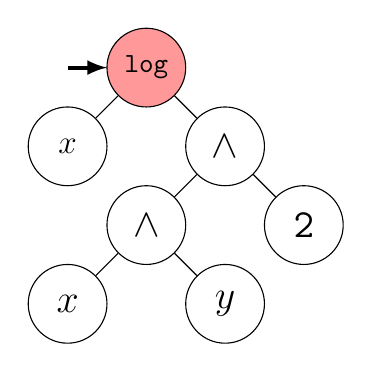
\begin{tikzpicture}[scale=0.5]
            \node [circle,draw,minimum width=1cm,fill=red!40] (Log) at (0,0) {\ttfamily log};
            \node [circle,draw,minimum width=1cm] (x1) at (-2,-2) {\large $x$};
            \node [circle,draw,minimum width=1cm] (pow1) at (2, -2) {\Large $\pow$};
            \node [circle,draw,minimum width=1cm] (pow2) at (0, -4) {\Large $\pow$};
            \node [circle,draw,minimum width=1cm] (x2) at (-2, -6) {\Large $x$};
            \node [circle,draw,minimum width=1cm] (y) at (2, -6) {\Large $y$};
            \node [circle,draw,minimum width=1cm] (2) at (4, -4) {\Large \ttfamily 2};
            
            \draw [-latex, line width=0.05cm](-2,0) -- (-1,0);
            \draw (Log) -- (x1);
            \draw (Log) -- (pow1);
            \draw (pow1) -- (pow2);
            \draw (pow2) -- (x2);
            \draw (pow2) -- (y);
            \draw (pow1) -- (2);
        \end{tikzpicture} & 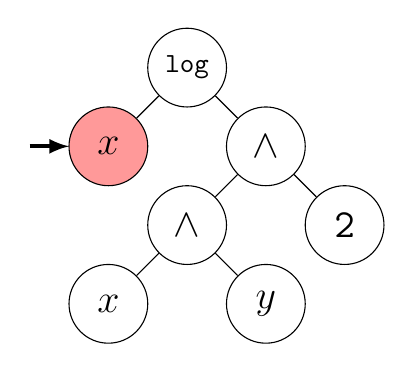
\begin{tikzpicture}[scale=0.5]
            \node [circle,draw,minimum width=1cm] (Log) at (0,0) {\ttfamily log};
            \node [circle,draw,minimum width=1cm,fill=red!40] (x1) at (-2,-2) {\Large $x$};
            \node [circle,draw,minimum width=1cm] (pow1) at (2, -2) {\Large $\pow$};
            \node [circle,draw,minimum width=1cm] (pow2) at (0, -4) {\Large $\pow$};
            \node [circle,draw,minimum width=1cm] (x2) at (-2, -6) {\Large $x$};
            \node [circle,draw,minimum width=1cm] (y) at (2, -6) {\Large $y$};
            \node [circle,draw,minimum width=1cm] (2) at (4, -4) {\Large \ttfamily 2};
            
            \draw [-latex, line width=0.05cm](-4,-2) -- (-3,-2);
            \draw (Log) -- (x1);
            \draw (Log) -- (pow1);
            \draw (pow1) -- (pow2);
            \draw (pow2) -- (x2);
            \draw (pow2) -- (y);
            \draw (pow1) -- (2);
        \end{tikzpicture} & 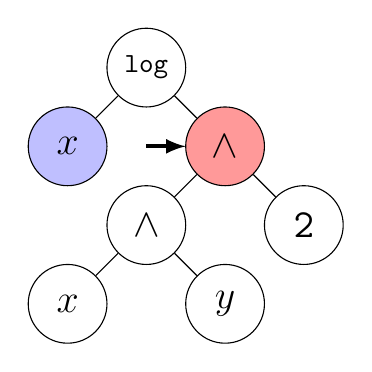
\begin{tikzpicture}[scale=0.5]
            \node [circle,draw,minimum width=1cm] (Log) at (0,0) {\ttfamily log};
            \node [circle,draw,minimum width=1cm,fill=blue!25] (x1) at (-2,-2) {\Large $x$};
            \node [circle,draw,minimum width=1cm,fill=red!40] (pow1) at (2, -2) {\Large $\pow$};
            \node [circle,draw,minimum width=1cm] (pow2) at (0, -4) {\Large $\pow$};
            \node [circle,draw,minimum width=1cm] (x2) at (-2, -6) {\Large $x$};
            \node [circle,draw,minimum width=1cm] (y) at (2, -6) {\Large $y$};
            \node [circle,draw,minimum width=1cm] (2) at (4, -4) {\Large \ttfamily 2};
            
            \draw [-latex, line width=0.05cm](0,-2) -- (1,-2);
            \draw (Log) -- (x1);
            \draw (Log) -- (pow1);
            \draw (pow1) -- (pow2);
            \draw (pow2) -- (x2);
            \draw (pow2) -- (y);
            \draw (pow1) -- (2);
        \end{tikzpicture} \\
        \hline
        $\log_x({(x^y)}^2)$&$x$&${(x^y)}^2$\\ 
        B.3.6 & B.3.2 & B.3.6 \\
        \hline \newpage \hline
        
        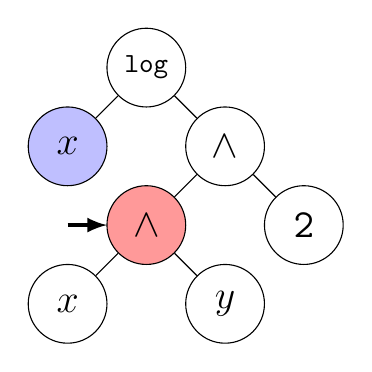
\begin{tikzpicture}[scale=0.5]
            \node [circle,draw,minimum width=1cm] (Log) at (0,0) {\ttfamily log};
            \node [circle,draw,minimum width=1cm,fill=blue!25] (x1) at (-2,-2) {\Large $x$};
            \node [circle,draw,minimum width=1cm] (pow1) at (2, -2) {\Large $\pow$};
            \node [circle,draw,minimum width=1cm,fill=red!40] (pow2) at (0, -4) {\Large $\pow$};
            \node [circle,draw,minimum width=1cm] (x2) at (-2, -6) {\Large $x$};
            \node [circle,draw,minimum width=1cm] (y) at (2, -6) {\Large $y$};
            \node [circle,draw,minimum width=1cm] (2) at (4, -4) {\Large \ttfamily 2};
            
            \draw [-latex, line width=0.05cm](-2,-4) -- (-1,-4);
            \draw (Log) -- (x1);
            \draw (Log) -- (pow1);
            \draw (pow1) -- (pow2);
            \draw (pow2) -- (x2);
            \draw (pow2) -- (y);
            \draw (pow1) -- (2);
        \end{tikzpicture} &  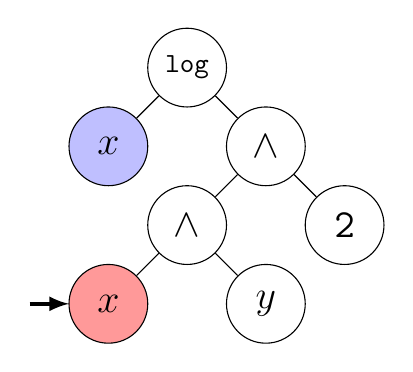
\begin{tikzpicture}[scale=0.5]
            \node [circle,draw,minimum width=1cm] (Log) at (0,0) {\ttfamily log};
            \node [circle,draw,minimum width=1cm,fill=blue!25] (x1) at (-2,-2) {\Large $x$};
            \node [circle,draw,minimum width=1cm] (pow1) at (2, -2) {\Large $\pow$};
            \node [circle,draw,minimum width=1cm] (pow2) at (0, -4) {\Large $\pow$};
            \node [circle,draw,minimum width=1cm,fill=red!40] (x2) at (-2, -6) {\Large $x$};
            \node [circle,draw,minimum width=1cm] (y) at (2, -6) {\Large $y$};
            \node [circle,draw,minimum width=1cm] (2) at (4, -4) {\Large \ttfamily 2};
            
            \draw [-latex, line width=0.05cm](-4,-6) -- (-3,-6);
            \draw (Log) -- (x1);
            \draw (Log) -- (pow1);
            \draw (pow1) -- (pow2);
            \draw (pow2) -- (x2);
            \draw (pow2) -- (y);
            \draw (pow1) -- (2);
        \end{tikzpicture} & 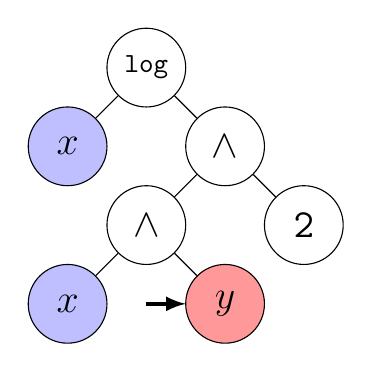
\begin{tikzpicture}[scale=0.5]
            \node [circle,draw,minimum width=1cm] (Log) at (0,0) {\ttfamily log};
            \node [circle,draw,minimum width=1cm,fill=blue!25] (x1) at (-2,-2) {\Large $x$};
            \node [circle,draw,minimum width=1cm] (pow1) at (2, -2) {\Large $\pow$};
            \node [circle,draw,minimum width=1cm] (pow2) at (0, -4) {\Large $\pow$};
            \node [circle,draw,minimum width=1cm,fill=blue!25] (x2) at (-2, -6) {\Large $x$};
            \node [circle,draw,minimum width=1cm,fill=red!40] (y) at (2, -6) {\Large $y$};
            \node [circle,draw,minimum width=1cm] (2) at (4, -4) {\Large \ttfamily 2};
            
            \draw [-latex, line width=0.05cm](0,-6) -- (1,-6);
            \draw (Log) -- (x1);
            \draw (Log) -- (pow1);
            \draw (pow1) -- (pow2);
            \draw (pow2) -- (x2);
            \draw (pow2) -- (y);
            \draw (pow1) -- (2);
        \end{tikzpicture}\\
        \hline
        $x^y$ & $x$ & $y$ \\
        B.3.6 & B.3.2 & B.3.2\\
        \hline
        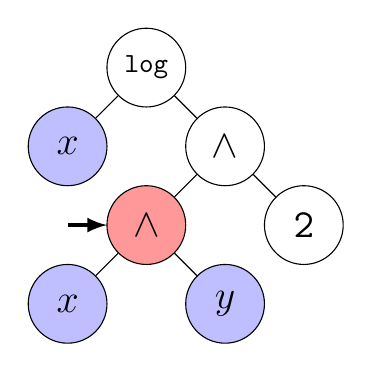
\begin{tikzpicture}[scale=0.5]
            \node [circle,draw,minimum width=1cm] (Log) at (0,0) {\ttfamily log};
            \node [circle,draw,minimum width=1cm,fill=blue!25] (x1) at (-2,-2) {\Large $x$};
            \node [circle,draw,minimum width=1cm] (pow1) at (2, -2) {\Large $\pow$};
            \node [circle,draw,minimum width=1cm,fill=red!40] (pow2) at (0, -4) {\Large $\pow$};
            \node [circle,draw,minimum width=1cm,fill=blue!25] (x2) at (-2, -6) {\Large $x$};
            \node [circle,draw,minimum width=1cm,fill=blue!25] (y) at (2, -6) {\Large $y$};
            \node [circle,draw,minimum width=1cm] (2) at (4, -4) {\Large \ttfamily 2};
            
            \draw [-latex, line width=0.05cm](-2,-4) -- (-1,-4);
            \draw (Log) -- (x1);
            \draw (Log) -- (pow1);
            \draw (pow1) -- (pow2);
            \draw (pow2) -- (x2);
            \draw (pow2) -- (y);
            \draw (pow1) -- (2);
        \end{tikzpicture} &  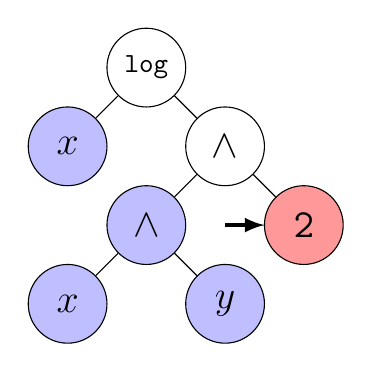
\begin{tikzpicture}[scale=0.5]
            \node [circle,draw,minimum width=1cm] (Log) at (0,0) {\ttfamily log};
            \node [circle,draw,minimum width=1cm,fill=blue!25] (x1) at (-2,-2) {\Large $x$};
            \node [circle,draw,minimum width=1cm] (pow1) at (2, -2) {\Large $\pow$};
            \node [circle,draw,minimum width=1cm,fill=blue!25] (pow2) at (0, -4) {\Large $\pow$};
            \node [circle,draw,minimum width=1cm,fill=blue!25] (x2) at (-2, -6) {\Large $x$};
            \node [circle,draw,minimum width=1cm,fill=blue!25] (y) at (2, -6) {\Large $y$};
            \node [circle,draw,minimum width=1cm,fill=red!40] (2) at (4, -4) {\Large \ttfamily 2};
            
            \draw [-latex, line width=0.05cm](2,-4) -- (3,-4);
            \draw (Log) -- (x1);
            \draw (Log) -- (pow1);
            \draw (pow1) -- (pow2);
            \draw (pow2) -- (x2);
            \draw (pow2) -- (y);
            \draw (pow1) -- (2);
        \end{tikzpicture} & 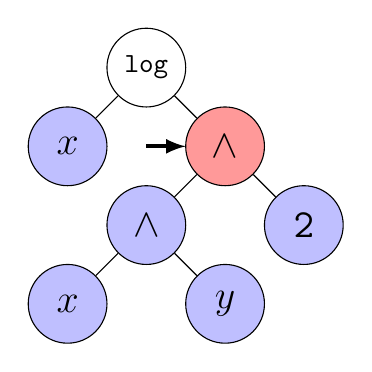
\begin{tikzpicture}[scale=0.5]
            \node [circle,draw,minimum width=1cm] (Log) at (0,0) {\ttfamily log};
            \node [circle,draw,minimum width=1cm,fill=blue!25] (x1) at (-2,-2) {\Large $x$};
            \node [circle,draw,minimum width=1cm,fill=red!40] (pow1) at (2, -2) {\Large $\pow$};
            \node [circle,draw,minimum width=1cm,fill=blue!25] (pow2) at (0, -4) {\Large $\pow$};
            \node [circle,draw,minimum width=1cm,fill=blue!25] (x2) at (-2, -6) {\Large $x$};
            \node [circle,draw,minimum width=1cm,fill=blue!25] (y) at (2, -6) {\Large $y$};
            \node [circle,draw,minimum width=1cm,fill=blue!25] (2) at (4, -4) {\Large \ttfamily 2};
            
            \draw [-latex, line width=0.05cm](0,-2) -- (1,-2);
            \draw (Log) -- (x1);
            \draw (Log) -- (pow1);
            \draw (pow1) -- (pow2);
            \draw (pow2) -- (x2);
            \draw (pow2) -- (y);
            \draw (pow1) -- (2);
        \end{tikzpicture}  \\
        \hline
        $x^y$ & $2$ & ${(x^y)}^2$ \\
        B.11.23 & B.3.2 & B.11.16 \\
        \hline
         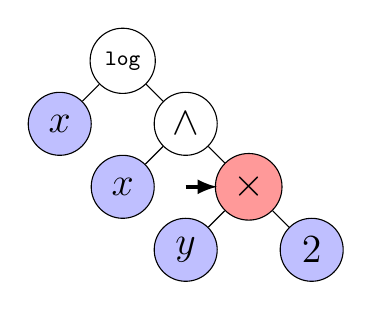
\begin{tikzpicture}[scale=0.4]
            \node [circle,draw,minimum width=0.8cm] (Log) at (0,0) {\ttfamily \footnotesize log};
            \node [circle,draw,minimum width=0.8cm,fill=blue!25] (x1) at (-2,-2) {\Large $x$};
            \node [circle,draw,minimum width=0.8cm] (pow) at (2, -2) {\Large $\pow$};
            \node [circle,draw,minimum width=0.8cm,fill=blue!25] (x2) at (0, -4) {\Large $x$};
            \node [circle,draw,minimum width=0.8cm,fill=red!40] (times) at (4, -4) {\Large $\times$};
            \node [circle,draw,minimum width=0.8cm,fill=blue!25] (y) at (2, -6) {\Large $y$};
            \node [circle,draw,minimum width=0.8cm,fill=blue!25] (2) at (6, -6) {\Large $2$};
            
            \draw [-latex, line width=0.05cm](2,-4) -- (3,-4);
            \draw (Log) -- (x1);
            \draw (Log) -- (pow);
            \draw (pow) -- (x2);
            \draw (pow) -- (times);
            \draw (times) -- (y);
            \draw (times) -- (2);
        \end{tikzpicture} & 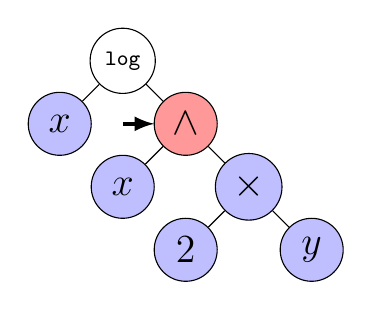
\begin{tikzpicture}[scale=0.4]
            \node [circle,draw,minimum width=0.8cm] (Log) at (0,0) {\ttfamily \footnotesize log};
            \node [circle,draw,minimum width=0.8cm,fill=blue!25] (x1) at (-2,-2) {\Large $x$};
            \node [circle,draw,minimum width=0.8cm,fill=red!40] (pow) at (2, -2) {\Large $\pow$};
            \node [circle,draw,minimum width=0.8cm,fill=blue!25] (x2) at (0, -4) {\Large $x$};
            \node [circle,draw,minimum width=0.8cm,fill=blue!25] (times) at (4, -4) {\Large $\times$};
            \node [circle,draw,minimum width=0.8cm,fill=blue!25] (2) at (2, -6) {\Large $2$};
            \node [circle,draw,minimum width=0.8cm,fill=blue!25] (y) at (6, -6) {\Large $y$};
            
            \draw [-latex, line width=0.05cm](0,-2) -- (1,-2);
            \draw (Log) -- (x1);
            \draw (Log) -- (pow);
            \draw (pow) -- (x2);
            \draw (pow) -- (times);
            \draw (times) -- (y);
            \draw (times) -- (2);
        \end{tikzpicture} &  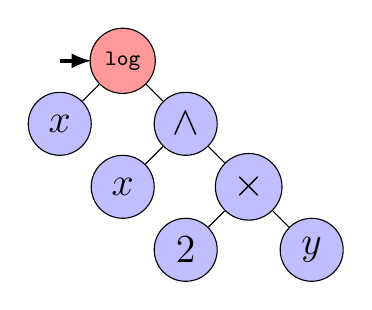
\begin{tikzpicture}[scale=0.4]
            \node [circle,draw,minimum width=0.8cm,fill=red!40] (Log) at (0,0) {\ttfamily \footnotesize log};
            \node [circle,draw,minimum width=0.8cm,fill=blue!25] (x1) at (-2,-2) {\Large $x$};
            \node [circle,draw,minimum width=0.8cm,fill=blue!25] (pow) at (2, -2) {\Large $\pow$};
            \node [circle,draw,minimum width=0.8cm,fill=blue!25] (x2) at (0, -4) {\Large $x$};
            \node [circle,draw,minimum width=0.8cm,fill=blue!25] (times) at (4, -4) {\Large $\times$};
            \node [circle,draw,minimum width=0.8cm,fill=blue!25] (2) at (2, -6) {\Large $2$};
            \node [circle,draw,minimum width=0.8cm,fill=blue!25] (y) at (6, -6) {\Large $y$};
            
            \draw [-latex, line width=0.05cm](-2,0) -- (-1,0);
            \draw (Log) -- (x1);
            \draw (Log) -- (pow);
            \draw (pow) -- (x2);
            \draw (pow) -- (times);
            \draw (times) -- (y);
            \draw (times) -- (2);
        \end{tikzpicture} \\
            \hline
          $y \times 2$ & $x^{2y}$& $\log_x(x^{2y})$ \\
          B.12.4 & B.11.23 & B.16.7 \\
          \hline
           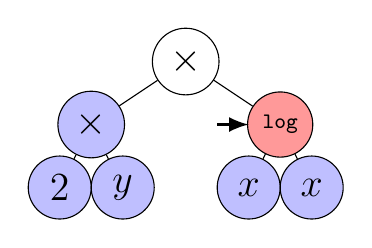
\begin{tikzpicture}[scale=0.4]
            \node [circle,draw,minimum width=0.8cm] (times1) at (0,0) {\Large $\times$};
            \node [circle,draw,minimum width=0.8cm,fill=blue!25] (times2) at (-3,-2) {\Large $\times$};
            \node [circle,draw,minimum width=0.8cm,fill=blue!25] (2) at (-4, -4) {\Large $2$};
            \node [circle,draw,minimum width=0.8cm,fill=blue!25] (y) at (-2, -4) {\Large $y$};
            \node [circle,draw,minimum width=0.8cm,fill=red!40] (log) at (3,-2) {\ttfamily \footnotesize log};
            \node [circle,draw,minimum width=0.8cm,fill=blue!25] (x1) at (2, -4) {\Large $x$};
            \node [circle,draw,minimum width=0.8cm,fill=blue!25] (x2) at (4, -4) {\Large $x$};

            
            \draw [-latex, line width=0.05cm](1,-2) -- (2,-2);
            \draw (times1) -- (times2);
            \draw (times2) -- (2);
            \draw (times2) -- (y);
            \draw (times1) -- (log);
            \draw (log) -- (x1);
            \draw (log) -- (x2);
        \end{tikzpicture} & 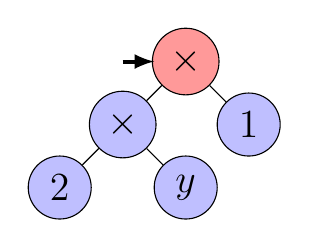
\begin{tikzpicture}[scale=0.4]
            \node [circle,draw,minimum width=0.8cm,fill=red!40] (times1) at (0,0) {\Large $\times$};
            \node [circle,draw,minimum width=0.8cm,fill=blue!25] (times2) at (-2,-2) {\Large $\times$};
            \node [circle,draw,minimum width=0.8cm,fill=blue!25] (2) at (-4, -4) {\Large $2$};
            \node [circle,draw,minimum width=0.8cm,fill=blue!25] (y) at (0, -4) {\Large $y$};
            \node [circle,draw,minimum width=0.8cm,fill=blue!25] (1) at (2,-2) {\Large $1$};

            
            \draw [-latex, line width=0.05cm](-2,0) -- (-1,0);
            \draw (times1) -- (times2);
            \draw (times2) -- (2);
            \draw (times2) -- (y);
            \draw (times1) -- (1);
        \end{tikzpicture} &
        
        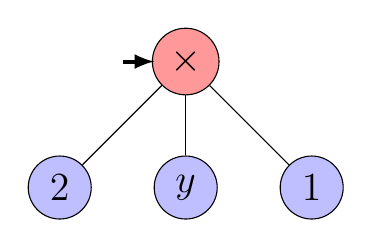
\begin{tikzpicture}[scale=0.4]
            \node [circle,draw,minimum width=0.8cm,fill=red!40] (times) at (0,0) {\Large $\times$};
            \node [circle,draw,minimum width=0.8cm,fill=blue!25] (2) at (-4, -4) {\Large $2$};
            \node [circle,draw,minimum width=0.8cm,fill=blue!25] (y) at (0, -4) {\Large $y$};
            \node [circle,draw,minimum width=0.8cm,fill=blue!25] (1) at (4,-4) {\Large $1$};

            
            \draw [-latex, line width=0.05cm](-2,0) -- (-1,0);
            \draw (times) -- (2);
            \draw (times) -- (y);
            \draw (times) -- (1);
        \end{tikzpicture} \\
        \hline
        $\log_x(x)$ & $(2y)\times 1$ & $2y1$\\
        B.16.5&B.12.12&B.12.2\\
        \hline
        \newpage
        \hline
        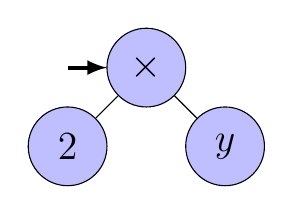
\begin{tikzpicture}[scale=0.5]
            \node [circle,draw,minimum width=1cm,fill=blue!25] (times) at (0,0) {\Large $\times$};
            \node [circle,draw,minimum width=1cm,fill=blue!25] (2) at (-2, -2) {\Large $2$};
            \node [circle,draw,minimum width=1cm,fill=blue!25] (y) at (2, -2) {\Large $y$};

            
            \draw [-latex, line width=0.05cm](-2,0) -- (-1,0);
            \draw (times) -- (2);
            \draw (times) -- (y);
        \end{tikzpicture}&& \\
        \hline
        $2y$&&\\
        B.12.20&&\\
        \hline
        \end{longtable}
    \end{center}

Then, $\Autosimplify(\log_x({(x^y)}^2)) = 2y$.
\end{exa}

\subsection{Implementation Details}

Most of the Lua implementation of autosimplification is straightforward. The {\fontfamily{qcr}\selectfont autosimplify} method is part of the expression ``interface", and each kind of expression implements its own transformations for autosimplification, calling {\fontfamily{qcr}\selectfont autosimplify} on any subexpressions first if the expression is a compound expression.

\inputminted[
firstline=113,
lastline=135,
breaklines]
{lua}
{core/binaryoperation.lua}



Simplifying products and sums works a little differently in the implementation then Definition \ref{def6} would suggest. Elements of product or sum expressions are compared two at a time, and sorted as ring properties are applied to them. This is for efficiency purposes, so we don't have to sort the list of terms first and then go back over the list and apply each property. In particular, B.12.16 and B.13.14 require comparing every element in the list to every other element even if the list is sorted on $\lhd$, so this reduces the runtime of each step of sum and product simplification from $O(n^2)$ to $O(n\log(n))$, where $n$ is the number of subexpressions.

One noteworthy part of autosimplification is rational power simplification - that is, transforming expressions like $\sqrt{8}$ into $2\sqrt{2}$. The core part of the transformation takes the prime factorization of the base (assuming the base is an integer) and applies transformation $\spow$.17, then factors out the largest integer power of each prime factor and leaves the remaining part in radicals. Prime factorization, even using the Pollard-Rho algorithm like our CAS does, is still slow, so autosimplification will only attempt rational power simplification if the base is small enough - by default, this is $10^{7}$ - the square root of the maximum integer that can be represented in a single digit by the big number library.

\inputminted[
firstline=78,
lastline=127,
breaklines]
{lua}
{core/binaryoperation/power.lua}

\newpage

\section{Symbolic Root-Finding of Polynomials}

Numeric methods have long been the dominant approach for root finding for scientific purposes, in part because exact formulas for the roots of many kinds of functions do not exist. However, exact solutions, if they exist, are easier to compute to a large precision, and are a common feature of computer algebra systems. In this section, we describe a method for finding the exact roots of univariate polynomials if they can be written in terms of radicals.

\subsection{Polynomial Rings}

\begin{defin} \label{def7}
    Let $R$ be a ring and $x$ be a symbol. The \emph{polynomial ring} $R[x]$ constructed from $R$ is the set of all elements of the form
    
    \begin{equation*}
        a_0 + a_1x + a_2x^2 + \ldots + a_nx^n = \sum_{i=0}^na_ix^i
    \end{equation*}
    
    where all $a_i \in R$, and $n \in \mathbb{N}$.  An element of $R[x]$ is a \emph{polynomial}, and an element of each of the $a_i$ are the polynomial's \emph{coefficients}. If the coefficients, say $\{a_{n}, a_{n-1}, \ldots, a_{k+1}\}$ are all zero elements of $R$, this polynomial is the same element as $\sum_{i=0}^ka_ix^i$. 
    
     Polynomial ring addition and ring multiplication are defined as is expected for symbolic manipulations. For polynomials $p, q \in R[x]$, if $p = \sum_{i=0}^{n}a_ix^i$ and $q = \sum_{i=0}^{m}b_ix^i$,
    
    \begin{equation*}
        p + q = \sum_{i=0}^{\max\{m,n\}} (a_i+b_i)x^i
    \end{equation*}
    
    and
    
    \begin{equation*}
        p \times q = \sum_{i=0}^{m + n} 
        (\sum_{j=0}^{i}a_jb_{i-j}) x^i.
    \end{equation*}
    
    Generally, there is no risk of ambiguity between operations in $R$ and operations in $R[x]$, so we use $+$ and $\times$ to refer to addition and multiplication in both rings.
    
    \begin{defin}
        If $R$ is a ring, $R[x]$ is a polynomial ring, and \[p=\sum_{i=0}^na_ix^i \in R[x]\] with $a_n \neq 0$, $n$ is the \emph{degree} of $p$, denoted $\deg(p) = n$. Also, $a_n$ is the \emph{leading coefficient} of $p$, denoted $a_n = \lc(p)$. If $\lc(p) = 1$, $p$ is \emph{monic}.    \end{defin}
    
    \begin{exa}
        Consider the polynomial ring $\mathbb{Q}[x][y]$. This is a \emph{multivariate polynomial ring}, and elements in the ring are \emph{multivariate polynomials}, since more than one symbol can appear in the polynomial. If only a single symbol can appear in a polynomial, the ring and polynomials are \emph{univariate} instead. According to Definition \ref{def7}, the expression \[p = (x^2+ 3x+1)y^2 + (x^3 + 6x)y + (12x + 8)\] is an element of $\mathbb{Q}[x][y]$. Typically, though, we allow any expression that is semantically equal to a polynomial to represent the same element of a polynomial ring, so we can represent $p$ as \[x^2y^2+3xy^2 + y^2 + x^3y + 6xy + 12x + 8\]
        or even as
        \[(y)x^3 + (y^2)x^2 + (3y^2 + 6y + 12)x + (y^2 + 8),\] an element of $\mathbb{Q}[y][x]$.
        
        This example illustrates a general rule: multivariate polynomial rings with exact same symbols are isomorphic regardless of the order with which the rings are constructed. If $R$ is the base ring and $S = \{x_1,\ldots, x_k\}$ are the symbols used to construct the polynomial ring, we write $R[x_1, \ldots, x_k]$ to represent the full polynomial ring as a subset of $\mathcal{X}(S, R, \{+, \times, \pow\})$ without ambiguity.
        
        However, the degree and leading coefficients of such polynomials are now ambiguous. When dealing with multivariate polynomials, we typically remedy this by using a second argument to specify the last symbol used to construct the ring. So,
        
        \[\deg(p, x) = 3, \deg(p, y) = 2, \lc(p, x) = y, \text{ and } \lc(p, y) = x^2+3x+1.\]

    \end{exa}
    
    While a polynomial ring is never a field, the following still holds:
    
    \begin{thm}
        If $R$ is a field, $R[x]$ is an Euclidean domain.
    \end{thm}
    
    \begin{thm}
        If $R$ is a commutative ring, $R[x]$ is also commutative.
    \end{thm}
    
    \begin{defin}
        Let $R$ be a ring, $R[x]$ be a polynomial ring, and $p \in R[x]$. The \emph{evaluation} of a polynomial at a point $a \in R$ is the result of replacing each occurrence of $x$ in $p$ with $a$ and calculating. In other words, evaluation is a function $f$ from $R$ to $R$ defined by $f(a) = \subs(p, \{(x, a)\})$.
    \end{defin}
    
    Then, finding the roots of a polynomial are equivalent to finding when the evaluation of a polynomial is zero. However, this is dependent on the underlying ring $R$. For instance, the polynomial $x^2-2$ has no roots in $\mathbb{Q}[x]$, but it does have roots in $\mathbb{R}[x]$ and $\mathbb{C}[x]$, namely $\pm\sqrt{2}$. The polynomial $x^2+2$ does not have roots in $\mathbb{Q}[x]$ or $\mathbb{R}[x]$, but it does in $\mathbb{C}[x]$, namely $\pm\sqrt{2}i$.
    
    In fact, due to the fundamental theorem of algebra, any polynomial in $\mathbb{Q}[x]$ or $\mathbb{R}[x]$ is guaranteed to have roots in $\mathbb{C}[x]$. By definition, this makes the field $\mathbb{C}$ an \emph{algebraic extension} of the fields $\mathbb{Q}$ and $\mathbb{R}$.
    
    A symbolic-root finding algorithm over $\mathbb{Q}[x]$ starts with finding a factorization of the polynomial, since, if the evaluation of any factor is zero, the overall polynomial's evaluation is zero.
    
\end{defin}

\subsection{Factorization}


    Given a ring $R$ and an element $x \in R$, a \emph{factorization} of $x$ is a list of elements $(x_1, \ldots ,x_n)$ such that $x_1\cdots x_n = x$. If $R$ is commutative, like all of the rings we encounter in this section, then factorizations are equivalent no matter what order the elements are multiplied in.
    
    In a field, factorizations are unintresting, since we can simply add an element and its multiplicative inverse to the factorization and get another factorization. However, this problem is still present even if $R$ is not a field, as long as there exist some elements that have inverses (a quick check shows $1$ is always its own inverse in any ring).
    
    \begin{defin}
        A \emph{unit} $u$ of a ring $R$ is an invertible element, i.e, there exists some $v \in R$ for which $uv = vu = 1$.
    \end{defin}
    
    In a field $F$, every non-zero element is a unit. In a polynomial ring $F[x]$ constructed from a field $F$, the units are the non-zero degree $0$ polynomials, that is, all of the elements of $F$ except $0$. 
    
    \begin{defin}
        A non-zero element $x$ of a ring $R$ is \emph{irreducible} if there exists no factorization of $x$ with more than 1 element that is not a unit. An \emph{irreducible factorization} of a non-zero element $x$ is a factorization $ux_1..x_n$ such that each $x_i$ is an irreducible element that is not a unit, and $u$ is a unit.
    \end{defin}
    
    In other words, an irreducible factorization breaks an element of a ring into as many factors as possible up to the units of that ring.
    
    \begin{exa}
        Consider the ring of integers $\mathbb{Z}$. The element 30 is not irreducible, since it can be factored as $(6)(5)$. This is not an irreducible factorization, though, since $6$ can be factored as $(2)(3)$. This means $(2)(3)(5)$ is an irreducible factorization of 30. Of course, $(-1)(-2)(3)(5)$ and $(-2)(-3)(5)$ are as well. 
        
        Typically, we decide on a canonical irreducible factorization over a ring that is completely unique including the units and is dependent on the ring itself. For the integers, this can be done by ensuring each non-unit factor is positive and adding a single $-1$ if needed, so $(2)(3)(5)$ is the canonical irreducible factorization of 30. Positive irreducible elements of $\mathbb{Z}$ are better known as prime numbers.
    \end{exa}
    
    \begin{defin}
        A \emph{unique factorization domain} is an integral domain $R$ such that every non-zero non-unit element $x \in R$ has a unique irreducible factorization up to the units of $R$. 
    \end{defin}
    
    It can be difficult to determine whether irreducible factorization are unique in an arbitrary ring. Fortunately, we can use the following theorems to help:
    
    \begin{thm}[\cite{aa},Theorem 21.7]
        If $R$ is a Euclidean domain, $R$ is a unique factorization domain.
    \end{thm}
    
    \begin{thm}[\cite{aa},Theorem 21.6]
        If $R$ is a unique factorization domain, $R[x]$ is a unique factorization domain.
    \end{thm}
    
    This means that $\mathbb{Z}$, $\mathbb{Z}[x]$, and even multivariate polynomial rings constructed from $\mathbb{Z}$ and $\mathbb{Q}$ are all unique factorization domains.
    
    The following chain of subsets summarizes the relationships between various kinds of rings:
    \begin{center}
        Fields $\subseteq$ Euclidean Domains $\subseteq$ Unique Factorization Domains $\subseteq$ \\ Integral Domains $\subseteq$ Commutative Rings $\subseteq$ Rings
    \end{center}
    
    In this and the following subsections, we develop an algorithm for finding the irreducible factorization of any non-zero polynomial over $\mathbb{Q}[x]$. We use this algorithm to build a symbolic root-finding algorithm over $\mathbb{Q}[x]$, including solutions that are not rational or real numbers.
    
    
    \subsubsection{Square-free factorization in $\mathbb{Q}[x]$}
    
    \begin{defin}
        Given a ring $R$, an element $x \in R$ is \emph{square-free} if it has an irreducible factorization
        
        \begin{equation*}
            x = ux_1 \cdots x_n
        \end{equation*}
        
        where all $x_1, \ldots , x_n$ are distinct.
    \end{defin}
    
    Typically, when $x$ is not square-free, we use powers to denote repeated factors as a shorthand. An equivalent statement is that there does not exist a non-unit element $y \in R$ such that $y^2\mid x$.
    
    
    \begin{defin}
        Given a Euclidean domain $R$ and an element $x \in R$, if
        
        \begin{equation*}
            x = us_1\cdots s_m^m
        \end{equation*}
        
        where each $s_1, \ldots , s_m$ is relatively prime and square-free, $us_1\cdots s_m^m$ is a \emph{square-free factorization} of $x$. 
    \end{defin}
    
    \begin{exa}
        Given the ring $\mathbb{Q}[x]$, the polynomial \[ p = x^3+x+\frac{1}{2}\] is square-free, as it is irreducible. The polynomial \[ q = {x}^{5}+{\frac {137}{6}}{x}^{4}+{\frac {493}{3}}{x}^{3}+296{x}^{
2}-{\frac {1600}{3}}x+{\frac{512}{3}} \] is not square free, since its irreducible factorization is \[\left( x-\frac{1}{2}\right)\left(x-\frac{2}{3}\right)(x+8)^3 \].

    The square-free factorization of $q$ is the same as its irreducible factorization, except the first two terms are multiplied together, \[q = \left(x^2-\frac{7}{6}x+\frac{1}{3}\right)(x+8)^3.\]
    \end{exa}
    
    The factorization of polynomials in $\mathbb{Q}[x]$ starts with performing a square-free factorization. We use the following theorem to motivate an efficient algorithm for square-free factorization:
    
    \begin{thm} \label{thm1}
        Let $p \in \mathbb{Q}[x]$, and let $p' \in \mathbb{Q}[x]$ be the formal derivative of $p$. Then, $p$ is square free if and only if $\gcd(p(x), p'(x)) = 1$.
    \end{thm}
    
    \begin{proof}
          ($\implies$) Assume $\gcd(p(x), p'(x)) \neq 1$. Then, there exists a polynomial $k \in \mathbb{Q}[x]$ of degree greater than $0$ such that $p = ku$ and $p' = kv$ for some $u, v \in \mathbb{Q}[x]$, so 
         \begin{align*}
             p' = k'u + ku' = kv & \iff k'u = k(v-u')\\
                                 & \iff u = \frac{k(v-u')}{k'}\\
                                 & \iff p = \frac{k^2(v-u')}{k'}
         \end{align*}
         
         If $k'\mid (v-u')$, then $k^2\mid p$, and $p$ is not square free. Otherwise, $k'\mid k$ and  $\deg(k') > 0$, so $p = k'wu$ and $p = k'wv$ for some $w \in \mathbb{Q}[x]$. Then, repeat this process with $k = k'$, $u = wu$, and $v = wv$ while $k'\mid k$. Since $\deg(k') < \deg(k)$, at some point this process terminates, and $p$ is not square-free.
         
         \hspace{0pt}
         
         ($\impliedby$) Assume $p$ is not square-free, so $p = k^2u$ for some $k, u \in \mathbb{Q}[x]$ such that $\deg(k) > 0$. Then, $p' = 2kk'u + k^2u' = k(2k'u+ku')$, so $k\mid p$ and $k\mid p'$, and $\gcd(k, k') > 1$.
    \end{proof}
    
    The core of the square-free factorization algorithm on a polynomial $p$ is to repeatedly find the gcd of $p$ and $p'$, and divide $p$ by that gcd. First, though, we divide $p$ by its leading coefficient to get the unit $u$ in the square-free factorization.
    
    \begin{algorithm}\small
    \caption{Yun's Square-Free Factorization Algorithm \cite{yun}}
        \begin{algorithmic}[1]
            \Require $p \in \mathbb{Q}[x]$ (or $p \in \mathbb{F}[x]$ where $F$ is a field and $\mathbb{Z} \subseteq X$) and $p \neq 0$
            \State $P \gets p/\lc(p, x)$
            \State $S \gets \lc(p, x)$ as Expression
            \State $R \gets \gcd(P, P')$
            \State $F \gets \frac{P}{R}$
            \State $i$ \gets 1
            \While{$R \neq 1$}
                \State $G \gets \gcd(R, F)$
                \State $s \gets F / G$
                \State $S \gets S \times s^j$
                \State $R \gets R / G$
                \State $F \gets G$
                \State $i \gets i + 1$
            \EndWhile
            \State $S \gets S \times F^j$
            \State \Return $S$
        \end{algorithmic}
    \end{algorithm}
    
    While most operations are standard ring operations in $\mathbb{Q}[x]$, the operations on lines with the returned expression $S$ are expression operations (lines 2, 9, and 14), so the structure of the factorization is kept.
    
    \begin{exa}
        Let 
        \[ p = {x}^{5}+{\frac {137}{6}}{x}^{4}+{\frac {493}{3}}{x}^{3}+296{x}^{
2}-{\frac {1600}{3}}x+{\frac{512}{3}} \in \mathbb{Q}[x].\] 
Then, we start with $P = p$ and $S = 1$ so that 
\[ P' = 5{x}^{4}+{\frac {274}{3}}{x}^{3}+493{x}^{2}+592\,x-{\frac{1600}{
3}}.\] 
Then $R = \gcd(P, P') = x^2+16x+64$ and 
\[ F = x^3+\frac{41}{6}(x^2)-9x+\frac{8}{3}.\] 
Then, we enter the while loop, and the values are tabulated below:
\begingroup
\renewcommand*{\arraystretch}{2}
\begin{center}
    \begin{tabular}{c|c|c|c}
     Interation $i$ & $G$ & $S$ & $R$ \\
     \hline
     1 & $x+8$ & $1\left(x^2-\frac{7}{6}x+\frac{1}{3}\right)^1$ &  $x+8$ \\
     2 & $x+8$ & $1\left(x^2-\frac{7}{6}x+\frac{1}{3}\right)^1(1)^2$ & $1$ \\
    \end{tabular}
\end{center}
\endgroup

Finally, we take $F^3 = (x+8)^3$ as the final term of our factorization, and, after autosimplifying the result, we get $(x^2-\frac{7}{6}x+\frac{1}{3})(x+8)^3$ as the square-free factorization of $P$.
\end{exa}
    
    
    \subsubsection{From $\mathbb{Q}[x]$ To  $\mathbb{Z}[x]$}
    
    The algorithm we develop in the following sections only applies to square-free polynomials in $\mathbb{Z}[x]$, however, we can easily expand its results to factor any polynomial in $\mathbb{Q}[x]$. The first step is, given a polynomial $p \in Q[x]$, let $q = \frac{1}{c}p$, where $c$ is the least common multiple of the denominators of the coefficients of $p$. Then, $p = cq$, and $q \in \mathbb{Z}[x]$.
    
    \begin{defin}
        Given a polynomial $p$ in $R[x]$, where $R$ is a Euclidean domain, {\color{red} then} the gcd of the coefficients of $p$ is referred to as the \emph{content} of $p$, or $\cont(p)$. If $\cont(p) = 1$, $p$ is \emph{primitive} in $R[x]$. 
    \end{defin}
    
    We can now use one of many results named Gauss's Lemma:
    
    \begin{lemma}[\itshape Gauss]
        Let $p \in \mathbb{Q}[x]$. Then, $p$ is irreducible in $\mathbb{Z}[x]$ if and only if $p$ is primitive in $\mathbb{Z}[x]$ and irreducible in $\mathbb{Q}[x]$.
    \end{lemma}
    
    \begin{corollary} \label{cor1}
        Let $p = p_1\cdots p_n$ be an irreducible factorization of primitive $p$ in $\mathbb{Z}[x]$. Then, $p_1\cdots p_n$ is also an irreducible factorization in $\mathbb{Q}[x]$.
    \end{corollary}
    
    From Corollary \ref{cor1}, we can be confident that Algorithm 3.22 does successfully perform a complete decomposition of any polynomial in $\mathbb{Q}[x]$, granted $\zass$ can completely decompose square-free polynomials in $\mathbb{Z}[x]$.
    
    \begin{algorithm} \label{alg2}
    \caption{Factorization Algorithm Over $\mathbb{Q}[x]$}
        \begin{algorithmic}[1]
            \Require $p \in \mathbb{Q}[x]$ and $p \neq 0$
            \State $S$ \gets
            $\text{SquareFreeFactor}(p)$
            \State $F \gets 1$ as Expression
            \State $c \gets \subtree(S, 1)$
            \For{$i \in \{2, \ldots, \args(S)\}$}
                \State $T \gets \subtree(\subtree(S, i),1)$
                \State $e \gets \subtree(\subtree(S, i),2)$
                \State $d$ \gets lcm of the denominators of the coefficients of $T$
                \State $c \gets c \times d$
                \State $T \gets \frac{T}{d}$
                \State $I \gets \zass(T)$
                \For{$i \in \{1, \ldots, \args(I)\}$}
                    \State $F \gets F \times \subtree(I, i)^p$
                \EndFor
            \EndFor
            \State \Return $c \times F$
        \end{algorithmic}
    \end{algorithm}
    
    \subsubsection{Irreducible factorization in $\mathbb{Z}_p[x]$}
    
    We can also construct polynomial rings out of the modular arithmetic rings, $\mathbb{Z}_n$. Since these rings are only fields when $n$ is prime, we only consider the polynomial rings $\mathbb{Z}_p[x]$ for $p$ prime in this algorithm.  The factorization of polynomials in $\mathbb{Z}[x]$ is closely related to factorization in $\mathbb{Z}_p[x]$.
    
    Since we view $\mathbb{Z}_p$ as a field over the elements $\{0, 1,\ldots, p-1\}$ rather than congruence classes, we use the $=$ for equality rather than the traditional $\equiv$ when working with modular arithmetic. 
    
    There are oddities in factoring polynomials over finite fields compared to the integers. For instance, consider Fermat's Little Theorem:
    
    \begin{center}
        For any $x \in \mathbb{Z}_p$, $x^p = x$.
    \end{center}
    
    This implies every element of $\mathbb{Z}_p$ is a root of $x^p - x$, so the irreducible factorization of $x^p - x$ is \[x^p - x = (x)(x-1)(x-2) \cdots (x-(p-1)). \]
    
    The factorization algorithm we present, Berlekamp factorization, only works on monic, square-free polynomials in $\mathbb{Z}_p[x]$. Fortunately, Theorem \ref{thm1} applies to $\mathbb{Z}_p[x]$ in addition to $\mathbb{Q}[x]$. Unfortunately, square-free terms in $\mathbb{Z}[x]$ are not necessarily square-free in $\mathbb{Z}_p[x]$. This is since, if $q \in \mathbb{Z}_p[x]$ and $q' = 0$, $q$ need not be a constant. For instance, if $p = 3$, \[q = x^6 + 2x^3 + 1,\] so \[q' = 6x^5 + 6x^3 = 0,\] and thus $\gcd(q, q') = q \neq 1$. In the following section, we show the Zassenhaus Algorithm always hands monic, square-free polynomials to Berlekamp's algorithm. We can, however, also revise the square-free factorization algorithm to work over $\mathbb{Z}_p[x]$, so any polynomial in $\mathbb{Z}_p[x]$ is indeed capable of being factored if the user would need it.
    
    First, we need the the following theorem:
    
    \begin{thm}[\cite{casc1},Theorem 9.22]
        Let $q(x) \in \mathbb{Z}_p[x]$. Then, $q(x)^p = q(x^p)$.
    \end{thm}
    
    Assume $q \in \mathbb{Z}_p[x]$ is a monic, square-free polynomial with irreducible factorization $q = q_1\cdots q_n$. The core of the algorithm relies on an extension of the Chinese Remainder Theorem:
    
    \begin{thm}[\cite{casc1},Theorem 9.26(1)] \label{thm2}
        If $q = q_1\cdots q_n \in \mathbb{Z}_p[x]$, and $a_1, \ldots, a_n \in \mathbb{Z}_p[x]$, then there exists a unique polynomial $h$ with $\deg(h) \leq \deg(q)$ that satisfies \[h \textbf{ mod } u_i = a_i\] for all $1\leq i \leq n$.
    \end{thm}
    
    Each $a_i$ is called an \emph{auxiliary polynomial}. Once we know $h$, we use the following theorem to find factors of $q$:
    
    \begin{thm}[\cite{casc1},Theorem 9.26(2)] \label{thm3}
        Let $u, h \in \mathbb{Z}_p[x]$ from Theorem \ref{thm2}. Then, \[ u = \prod_{j=0}^{p-1}\gcd(u, h - j).\]
    \end{thm}
    
    Of course, we can't calculate $h$ directly, since we don't know the irreducible factors of $h$. Instead, we set up a system of equations to solve for $h$. This will not be an independent system, as $h$ varies with the choice of auxiliary polynomials. Fortunately, the basis vectors of the solution space can be used to find the irreducible factors of $u$ as per Theorem \ref{thm3}.
    
    
    The following theorem is the basis for the system of equations:
    
    \begin{thm}[\cite{casc1},Theorem 9.28] \label{thm4}
        Let $u, h \in \mathbb{Z}_p[x]$ such that $\deg(h) < \deg(u)$. Then, there exist $a_1, \ldots, a_n \in \mathbb{Z}_p[x]$ such that $h$ satisfies Theorem \ref{thm2} if and only if \[u\mid (h^p-h).\]
    \end{thm}
    
    To solve for the coefficients of an $h$ that satisfies Theorem \ref{thm2}, say,
    
    \[h = \sum_{j=0}^{d-1}h_jx^j,\]
    
    where $\deg(q) = d$, we know
    
    \begin{align*}
        h(x)^p-h(x) &= h(x^p)-h(x) \\
                    &= \sum_{j=0}^{d-1}h_j(x^{pj} -x^j).
    \end{align*}
    
    Since $\mathbb{Z}_p[x]$ is a Eucidean domain, there exist polynomials $Q_j$ and $r_j$ with \[ x^{pj} = Q_j(x)q(x)+r_j(x)\] such that $\deg(r_j) < \deg(q) = d$ for each $0 \leq j \leq d - 1$. Then,
    
    \begin{align*}
        h(x)^p-h(x)  &= \sum_{j=0}^{d-1}h_j(Q_j(x)q(x)+r_j(x) -x^j) \\
        &= \left(\sum_{j=0}^{n-1}h_jQ_j(x)\right)u(x) + \sum_{j=0}^{n-1}h_j(r_j(x) - x^j).
    \end{align*}
    
    Now, by Theorem \ref{thm4}, $h(x)^p-h(x) \textbf{ mod } q(x) = 0$, so 
    
    \begin{equation*}
        \sum_{j=0}^{n-1}h_j(r_j(x) - x^j) = 0.
    \end{equation*}
    
    Let $r_{ij}$ denote the coefficients of $r_j$, so \[ r_j(x) = \sum_{i=0}^{n-1}r_{ij}x^i.\] After substitution,
    
    \begin{equation*}
        \sum_{j=0}^{n-1}h_j(\sum_{i=0}^{n-1}r_{ij}x^i - x^j) = 0.
    \end{equation*}
    
    
    This is arranged into a system of linear equations. In matrix form, the equation is 
    
    \begin{align*}
        R\mathbf{h} = 0,
    \end{align*}
    
    where \[R_{ij} =  \begin{cases}
        r_{i-1,j-1} & i \neq j \\
        r_{i-1,j-1} -1 & i = j
    \end{cases},\] and $\mathbf{h}_i = h_{i-1}$. Each $r_{i,j}$ is computed as the $i$th coefficient of $x^{pj} \textbf{ mod } q(x)$, and we find a basis using a standard linear algebra null space solver.
    
    Before we present the full algorithm, we first provide an example for clarity. 
    
    \begin{exa}
    Let $q = x^7+4x^5+3x^2+2x+1 \in \mathbb{Z}_7[x]$. First, we calculate the remainders $x^{pj} \textbf{ mod } q(x)$ for $p$ from 0 to $\deg(q) - 1 = 6$:
    \begin{align*}
        r_0 = x^{0} \textbf{ mod } q(x) & = 1,\\
        r_1 = x^{7} \textbf{ mod } q(x) & = 3x^5 + 4x^2 + 5x + 6,\\
        r_2 = x^{14} \textbf{ mod } q(x) & = 6x^6 + 4x^5 + 5x^4 + 6x^3 + 3x^2 + 6x + 5, \\
        r_3 = x^{21} \textbf{ mod } q(x) & = x^6 + 4x^5 + 5x^4 + 6x^3 + 2x^2 + 5x + 6, \\
        r_4 = x^{28} \textbf{ mod } q(x) & =  2x^6 + 3x^5 + 4x^4 + 2x^2,\\
        r_5 = x^{35} \textbf{ mod } q(x) & = 4x^6 + 3x^5 + 2x^4 + 4x^3 + 6x^2 + 2x + 1, \text{ and}\\
        r_6 = x^{42} \textbf{ mod } q(x) & = 6x^5 + 5x^4 + 2x + 5.
    \end{align*}
    
    Column $i$ of the $R$ matrix corresponds to the coefficients of the polynomial $r_{i-1}$:
    
    
    \[R = \begin{bmatrix} 
    1-1 & 6 & 5 & 6 & 0 & 1 & 5 \\
    0& 5 - 1 & 6 & 5 & 0 & 2 & 2 \\
    0& 4 & 3 - 1& 2 & 2 & 6 & 0 \\
    0& 0 & 6 & 6 - 1 & 0 & 4 & 0 \\
    0& 0 & 5 & 5 & 4 - 1 & 2 & 5 \\
    0& 3 & 4 & 4 & 3 & 3 -1 & 6 \\
    0& 0 & 6 & 1 & 2 & 4 & 0 - 1
    \end{bmatrix} =
    \begin{bmatrix} 
    0& 6 & 5 & 6 & 0 & 1 & 5 \\
    0& 4 & 6 & 5 & 0 & 2 & 2 \\
    0& 4 & 2& 2 & 2 & 6 & 0 \\
    0& 0 & 6 & 5 & 0 & 4 & 0 \\
    0& 0 & 5 & 5 & 3 & 2 & 5 \\
    0& 3 & 4 & 4 & 3 & 2 & 6 \\
    0& 0 & 6 & 1 & 2 & 4 & 6 
    \end{bmatrix}
    \]
    
    A basis for the null space of $R$ is:
    
    \begin{equation*}
        \mathbf{h}_1 =   \begin{bmatrix}
        1 \\ 0\\ 0\\ 4\\ 1\\ 5\\5
        \end{bmatrix},
                \mathbf{h}_2 =   \begin{bmatrix}
        0 \\1 \\0 \\2\\ 5\\ 1\\ 5
        \end{bmatrix},
        \mathbf{h}_3 =   \begin{bmatrix}
        0\\ 0\\ 1\\ 0\\ 3 \\1 \\ 0
        \end{bmatrix},
    \end{equation*}
    
    thus the polynomials \[ 5x^6+5x^5+x^4+4x^3+1, 5x^6+x^5+5x^4+2x^3+x, \text{ and } x^5+3x^4+x^2 \]
    
    form a basis for the possible $h$ polynomials, and there are 3 irreducible factors of $q$. Using the linear combination
    \[ \begin{aligned}
        h &= (5x^6+5x^5+x^4+4x^3+1) + (5x^6+x^5+5x^4+2x^3+x) +  (x^5+3x^4+x^2) \\
        &= 3x^6 + 2x^4 + 6x^3 + x^2 + x + 1
        \end{aligned} \] 
    and Theorem \ref{thm3}, we get:
    \begin{align*}
        \gcd(q, h) &= 1, \\
        \gcd(q, h-1) &= 1, \\
        \gcd(q, h-2) &= 1,\\
        \gcd(q, h-3) &= 1,\\
        \gcd(q, h-4) &= x^2+2x+2,\\
        \gcd(q, h-5) &= 1, \text{ and}\\
        \gcd(q, h-6) &= x + 5.
    \end{align*}
    So, after dividing $q$ by $x^2+2x+2$ and $x + 5$, the irreducible factorization of $q$ in $\mathbb{Z}_7[x]$ is \[ q= x^7+4x^5+3x^2+2x+1 = (x^2+2x+2)(x + 5)(x^4 + 6x^2 + 4x + 5).\]
    The only remaining hurdle is determining what linear combination of the basis vectors is needed to produce an irreducible factorization, as Theorem \ref{thm3} only guarantees $h$ produces some factorization of $q$. This is done in the FindFactors procedure.
    
    \begin{algorithm}\small
    \caption{Berlekamp Factorization \cite{bf}}
        \begin{algorithmic}[1]
            \Require $q \in \mathbb{Z}_p[x]$, $q$ is monic and square-free.
            \If{$\deg(q) < 1$}
                \State \Return q
            \EndIf
            \State $R$ \gets RMatrix($q$)
            \State $B$ \gets AuxillaryBasis($R$)
            \If{$|S| = 1$}
                \State \Return $q$
            \EndIf
            \State \Return FindFactors($q, B$)
        \end{algorithmic}
    \end{algorithm}
    
    The procedures RMatrix and AuxillaryBasis are ommited, the former being straightforward and the latter being outside the scope of this section. The FindFactors procedure is defined below. It essentially loops through the multiples of each term in the null space until it finds a factor of $q$, and then divides $q$ by that factor and continues dividing out both $q$ and the other factors until an irreducible factorization is found.
    
    \begin{algorithm}\small
    \caption{Find Factors}
        \begin{algorithmic}[1]
            \Require $q \in \mathbb{Z}_p[x]$, $q$ is monic and square-free.
            \Require $B$ is a set of basis of auxillary polynomials, $b \in \mathbb{Z}_p[x]$ and $\deg(b) < \deg(q)$ for all $b \in S$.
            \State $r \gets |B|$
            \State $F \gets \{u\}$
            \For{k \in \{2,\ldots,r\}}
               \State $b \gets S\{k\}$
               \State $oldF \gets F$
                \For{i \in $1, \ldots , \vert oldF \vert $}
                    \State $w \gets oldF\{k\}$
                    \State $j \gets 0$
                    \While{$j < p - 1$}
                        \State $g \gets gcd(b-j, w)$
                        \If{$g=1$}
                            \State $j \gets j + 1$
                        \ElsIf{$g = w$}
                            \State $j \gets p$
                        \Else
                            \State $F \gets F/\{w\}$
                            \State $t \gets w // g$
                            \State $F \gets F     \cup \{g, t\}$
                            \If{$|F| = r$}
                                \State \Return $F$
                            \Else
                                \State $j \gets j + 1$
                                \State $w = t$
                            \EndIf
                        \EndIf
                    \EndWhile
                \EndFor
            \EndFor
        \end{algorithmic}
    \end{algorithm}
    
    \end{exa}
    
    \newpage
    
    \subsubsection{Irreducible factorization in $\mathbb{Z}[x]$}
    
    The core of the Zassenhaus factorization algorithm is easier to descibe then the Berlekamp factorization algorithm. Zassenhaus factorization takes an irreducible factorization of a polynomial in $\mathbb{Z}_p[x]$ and uses \emph{Hensel lifting} (described later) to transform each factor to an appropriate factor in $\mathbb{Z}[x]$ if that factor is truly an irreducible factor in $\mathbb{Z}[x]$.

Our first order of business is to convert the polynomial to a monic polynomial so it can be fed to Berlekamp's algorithm. Unfortunately, $\mathbb{Z}$ is not a field, so we can't just divide each term in the polynomial by it's leading coefficient in general. Given a primitive polynomial \[a = \sum_{i=0}^{n}a_ix^i \in \mathbb{Z}[x],\] we construct the polynomial
\begin{align*}
     b &= a_n^{n-1}a(x/a^n) \\
       &= x^n + \sum_{i=0}^{n-1}a_n^{n-1-i}a_ix^i.
\end{align*}

Then, if $b$ has the irreducible factorization \[ b = f_1f_2\cdots f_r,\]

$a$ has the related irreducible factorization

\[ a = g_1(p_nx)g_2(p_nx)\cdots g_r(p_nx),\]

where each $g_i$ is a primitive polynomial obtained from dividing $f_i$ by the largest integer possible such that $g_i$ is still in $\mathbb{Z}[x]$, \[ g_i = \frac{f_i}{\cont(f_i)}.\] We refer to $g_i$ as the \emph{primitive part} of $f_i$. 

Now that we have a monic polynomial $b$ in $\mathbb{Z}[x]$, we convert it to $\mathbb{Z}_p[x]$. There is only one natural way to project from $\mathbb{Z}$ to $\mathbb{Z}_p$, which is to take the remainder of the element mod $p$. To project back to $\mathbb{Z}$, we choose a set of $p$ \emph{representatives} from $\mathbb{Z}$ that all have different remainders mod $p$. The \emph{non-negative representation} is the one used thus far, where  \[\mathbb{Z}_p = \{0, 1, \ldots , p-1\} .\] Zassenhaus factorization uses the \emph{symmetric representation}, \[\mathbb{Z}_p = \left\{\left\lfloor \frac{p-1}{2} \right\rfloor,\ldots , 0, \ldots, \left\lfloor \frac{p}{2} \right\rfloor\right\} ,\] to project from $\mathbb{Z}_p$ to $\mathbb{Z}$. The algebra is the same regardless of the chosen representatives, but it is clearer going forwards to use the symmetric representation.

Berlekamp factorization requires $b$ to be square-free as well as monic. To do this, we iterate through each prime $p$ and compute the gcd of the projection of $b$ onto $\mathbb{Z}_p[x]$ with its derivative until the gcd is 1 as per Theorem \ref{thm1}. The following theorem guarantees the process will terminate:

\begin{thm} [\cite{casc1},Theorem 9.55]
    Let $p$ be a prime and $u$ be a square-free polynomial in $\mathbb{Z}[x]$ such that $p \nmid \lc(u)$. Then, the projection of $u$ onto $\mathbb{Z}_p[x]$ is not square-free for a finite number of $p$.
\end{thm}

In general, polynomials in $\mathbb{Z}_p[x]$ factor into smaller components than polynomials in $\mathbb{Z}[x]$.

\begin{thm} [\cite{casc1},Theorem 9.42(1)]
    Let $u$ be a polynomial in $\mathbb{Z}_p[x]$. Then, the irreducible factorization of $u$ in $\mathbb{Z}_p[x]$ has the same or more non-unit factors than the irreducible factorization of $u$ in $\mathbb{Z}[x]$ using projection from $\mathbb{Z}_p[x]$ to $\mathbb{Z}[x]$.
\end{thm}

\begin{corollary}[\cite{casc1},Theorem 9.42(2)]
     Let $u$ be an irreducible polynomial in $\mathbb{Z}_p[x]$. Then, $u$ is irreducible in $\mathbb{Z}[x]$.
\end{corollary}

This means that if the Berlekamp algorithm returns a single factor of a polynomial, we terminate the algorithm immediately.

The complete Zassenhaus algorithm is defined below.

    \begin{algorithm}\small
    \caption{ZassenhausFactor \cite{zf}}
        \begin{algorithmic}[1]
            \Require $a \in \mathbb{Z}[x]$, $a$ is primitive
            \State $n \gets \deg(a)$
            \State $l \gets \lc(a)$
            \State $b \gets \subs(l^{n-1}u, (x, y/l))$
            \State $p$ \gets FindPrime($b$)
            \State $S$ \gets BerlekampFactor(InRing($b$,$\mathbb{Z}_p[y]$))
            \If{$\args(S) = 1$}
                \State \Return $a$
            \EndIf
            \State $k$ \gets FindMaxLifts($b$, $p$)
            \State $W$ \gets HenselLift($b$, $S$, $k$)
            \State $W \gets \subs(W, (y, lx))$
            \For{$i \in \{1, \ldots, \args(W)\}$}
                \State $\subtree(W, i) \gets \subtree(W, i)/\cont(W)$
            \EndFor
            \State \Return $W$
        \end{algorithmic}
    \end{algorithm}
    
The only part of the algorithm left to describe is the Hensel lifting, on line 10, and the calculation for the maximum number of Hensel lifting steps to perform, on line 9. Hensel lifting takes factors of a polynomial $b$ in $\mathbb{Z}_p$ and computes factors of $b$ in $\mathbb{Z}_{p^m}$ for successive $m = 2, 3, \ldots, k$. The value of $k$, the maximum number of times to perform Hensel lifting, can be determined using the following theorem:

\begin{thm}
    Let $b, f \in \mathbb{Z}[x]$ such that $f \mid b$ and $\deg(b) = n$. Then,
    \[ \max_{i \in \mathbb{N}} |a_i| \leq B = 2^n\sqrt{n+1}\max_{i \in \mathbb{N}} |f_i| \]
\end{thm}

The maximum absolute value of the coefficients of a polynomial is the \emph{height} of that polynomial. Since we are using the symmetric representation, to ensure that the coefficients of the factors of $b$ in $\mathbb{Z}_{p^m}[x]$ are large enough to be their own representatives in $\mathbb{Z}[x]$, we need to ensure they are less than $2B$, so Hensel lifting needs to be performed $\left\lceil \log_p(2B) \right\rceil$ times.

The Hensel lifting process uses an extension of Bezout's Lemma for polynomials. Given relatively prime polynomials $v_1, v_2, \ldots, v_s$ in a polynomial ring constructed from a field, $F[x]$, there exists polynomials $r_1, r_2, \ldots, r_s$ with each $\deg(r_i) < \deg(v_i)$ that satisfy \[1 = r_1{v_1}+r_2{v_2}+ \ldots +r_s{v_s}. \] From this equation, we can derive the following for any polynomial $P$:

\[P = \sigma_1\frac{v}{v_1}+\sigma_2\frac{v}{v_2}+ \ldots +\sigma_s\frac{v}{v_s}, \]

where $v = \prod_{i=1}^s(v_i)$, and $\deg(\sigma_i) < \deg(v_i)$ for each $\sigma_i$. This derivation makes use of the $r$ polynomials $r_i = F\sigma_i \textbf{ mod } v_i$.

In the first step of Hensel lifting, we use the Berlekamp factors as the $v_i$ terms. Otherwise, we use the factors from the previous step. First, we compute the difference between the current factorization in $\mathbb{Z}_{p^j}[x]$ and the actual polynomial $b \in \mathbb{Z}[x]$, \[E = u - v = u - \prod_{i=1}^s(v_i).\] If this difference is 0, then the factors are all the correct factors in $\mathbb{Z}[x]$, and we have found the irreducible factorization, so we can terminate the Hensel lifting process early! Otherwise, we compute

\[ F = E / p^{j-1}\]

in $\mathbb{Z}[x]$ and calculate the lifted factors for the next lift as

\[ v_i^* = v_i + p^{j-1}(F\sigma_i \textbf{ mod } v_i). \]

\begin{exa}
    Let $b = x^5-48x^4+720x^3-5760x^2+59904x-110592$. To obtain its irreducible factorization, since $b$ is monic and square-free, we jump straight to Berlekamp factorization with $p=11$. The irreducible factorization of $b$ in $\mathbb{Z}_{11}[x]$ is
    
    \[(x-5)(x+5)(x-2)(x^2-2x+4).\]
    
    Now, we calculate the maximum number of Hensel lifting steps $k$ as
    
    \[ k = \left\lceil \log_{11}(2B) \right\rceil = \left\lceil \log_{11}(2(2^5)(\sqrt{5+1})(110592)) \right\rceil \approx \left\lceil 6.95 \right\rceil  = 7.\]\
    
    The 7 steps of Hensel lifting, including the modulus and the $v_i$ polynomials at each step, are tabulated below.
    
    \begin{center}
        \begin{tabular}{|c|cccc|c|}
        \hline
            Step & \multicolumn{4}{c|}{Factors} & Modulus   \\
            \hline
             1&$(x-5)$ &$(x+5)$ &$(x-2)$& $(x^2-2x+4)$&11\\
             \hline
              2&$(x-5)$ &$(x+5)$ &$(x-2)$& $(x^2-24x+48)$&121\\
             \hline
                3&$(x-126)$ &$(x+126)$ &$(x-2)$& $(x^2-24x+48)$&1331\\
             \hline
                4&$(x-1457)$ &$(x+1457)$ &$(x-2)$& $(x^2-24x+48)$&14641\\
             \hline
                 5&$(x-30739)$ &$(x+30739)$ &$(x-2)$& $(x^2-24x+48)$&161051\\
             \hline
                 6&$(x-674943)$ &$(x+674943)$ &$(x-2)$& $(x^2-24x+48)$&1771561\\
             \hline
                 7&$(x-2868179)$ &$(x+2868179)$ &$(x-2)$& $(x^2-24x+48)$&19487171\\
             \hline
        \end{tabular}
    \end{center}

    The factors $(x-2)$ and $(x^2-24x+48)$ are true factors of $b$, which we can check by polynomial division. Perhaps obviously, $(x-2868179)$ and $(x+2868179)$ do not evenly divide $b$. In general, if Hensel lifting terminates at step $k$, the $v_i$ at step $k$ may not be the true factors of $b$. However, some partition of the factors will give the correct factors when the product of each partition set over $\mathbb{Z}_{p^k}[x]$ is taken. In this case, $(x-2868179)(x+2868179) = (x^2+96)$, which does in fact divide $b$. So, the irreducible factorization of $b$ is
    
    \[(x-2)(x^2-24x+48)(x^2+96).\]
\end{exa}

\subsection{Polynomial Decomposition}

Now that we have an irreducible factorization of a polynomial $p = cp_1\cdots p_n \in \mathbb{Q}[x]$, we can get the set of symbolic roots of $p$ by taking the union of the set of symbolic roots of each $p_i$. Each linear factor is of the form $ax+b$, so $x=-\frac{b}{a}$ is a root. There are exact formulas for the roots of polynomials of degree 2, 3, and 4 - the quadratic, cubic, and quartic formulas, respectively. It is not possible to write some roots of polynomials of degree 5 or higher using only addition, subtraction, multiplication, division, and exponentiation of rational numbers, so there can be no general formula for the roots of such polynomials.

However, the roots of some irreducible polynomials of degree 5 or higher may still be written using the symbols above (or our rational expression trees developed in appendix A). This is illustrated in the following example.

\begin{exa}
    The polynomial \[x^8 + 2x^4 - 1\] is irreducible over $\mathbb{Q}[x]$. However, by substituting $u=x^4$, we get the polynomial
    \[ u^2-u+1.\]
    
    The equation $u^2-u-1 = 0$ can be solved for $u$ using the quadratic formua, and has the roots \[ \left\{\frac{1+\sqrt{5}}{2}, \frac{1-\sqrt{5}}{2} \right\}.\] Substituting back gives the new quartic equations \[u^4 - \frac{1+\sqrt{5}}{2} = 0\] and 
    \[u^4 - \frac{1-\sqrt{5}}{2}=0,\]
    which can be solved exactly using the quartic formula or by converting to polar form.
\end{exa}

This method can also be used for some quartic polynomials with quadratic substitutions, which allows for the roots of those polynomials to be written in simpler form than the very long quartic formula. The general process is referred to as \emph{polynomial decomposition}. (Note that some authors use the term decomposition synonymously with factorization instead.)

\begin{defin}
    Let $p \in R[x]$ be a polynomial. Then, $p$ is \emph{decomposible} if there exists polynomials $p_1, \ldots, p_n$, called \emph{components}, all of degree greater than 1 such that
    \[p(x) = p_n(p_{n-1}(\cdots p_1(x)\cdots)) = p_n \circ p_{n-1} \circ \cdots \circ p_1.\]
    If no such decomposition exists, $p$ is \emph{indecomposable}. If each $p_i$ is indecomposable, $ p_n \circ \cdots  \circ p_1$ is said to be a \emph{complete decomposition} of $p$.
\end{defin}

In the above example, $(x^2-x+1)\circ(x^4)$ is a decomposition of $x^8 + 2x^4 -1$. A further decomposition is $(x^2-x+1)\circ(x^2)\circ(x^2)$. All polynomials of degree 3 or less are indecomposable, so this decomposition is complete.

Unlike irreducible polynomial factoring, complete decompositions are not unique up to units, although any two complete decompositions of a polynomial have the number of components and have the same degrees, possibly in a different order. For instance, $(x^2-2)\circ(x^2+1)\circ(x^2)$ and $(x^2-x+1)\circ(x^2)\circ(x^2)$ are unique decompositions of $x^8 + 2x^4 -1$.

The non-uniqueness of decompositions means we can ensure a decomposition of a paricular form exists. In particular, 

\begin{thm} \label{thm5}
    Let $p$ be a polynomial in $\mathbb{Q}[x]$. Then, $p$ can be decomposed as $p = A \circ b \circ C$, where
    \begin{enumerate}
        \item $\deg(C) < \deg(b \circ C) < \deg(p)$.
        \item $\deg(b \circ C) \mid  \deg(p, u)$.
        \item $(b \circ C)(0) = 0$.
        \item $(b \circ C) \mid (p(x)-p_0)$.
    \end{enumerate}
\end{thm}

This theorem can be used recursively to find a complete decomposition of a polynomial. Lines 1 and 2 of the below algorithm are used to ensure the decomposition satisfies the condition in Theorem \ref{thm5}(4). The set $S$ is obtained by irreducibly factoring $P$ and forming the set of products over all subsets of the factors of $P$.

The PolynomialExpand algorithm takes a polynomial in $\mathbb{Q}[x]$ and returns a polynomial in $\mathbb{Q}[x][t]$. It is defined below the decomposition algorithm.

\newpage

\begin{algorithm}\small
\caption{PolynomialDecompose}
    \begin{algorithmic}[1]
        \Require $p \in \mathbb{Q}[x]$
        \State $P \gets p - p_0$
        \State $S \gets $ The set of all nonconstant monic divisors of $P$
        \State $decomp \gets 1$
        \State $C \gets x$
        \While{$S \neq \emptyset$}
            \State $w \gets \arg \min_{s \in S}(\deg(s))$
            \State $S \gets S \setminus w$
            \If{$\deg(c) < \deg(w) < \deg(u)$ \AND $u\mid w$}
                \State $b \gets \text{PolynomialExpand}(w, C, t)$
                \State $A \gets \text{PolynomialExpand}(p, C, t)$
                \If{$\deg(b, x) = \deg(A, x) = 0$}
                    \State $decomp \gets \subs(b, \{(t,x)\}) \circ decomp$
                    \State $C \gets w$
                    \State $final \gets A$
                \EndIf
            \EndIf
            \EndWhile
            \If{$decomp=1$}
        \State \Return $p$
        \EndIf
        \State \Return $\subs(final, \{(t, x)\}) \circ decomp$
    \end{algorithmic}
\end{algorithm}

\begin{algorithm}\small
\caption{PolynomialExpand}
    \begin{algorithmic}[1]
        \Require $m,n \in \mathbb{Q}[x]$ and $t$ a symbol in $\mathcal{X}(S, A, F)$
        \State $q \gets m // n$
        \State $r \gets m \textbf{ mod } n$
        \State \Return $(t)(PolynomialExpand(q, n)) + r$
    \end{algorithmic}
\end{algorithm}



\subsection{Implementation Details \& Runtime Analysis}


As hinted at in the preceding sections, polynomials are generally represented in their own ring class and not as an expression tree. This class stores all of the coefficients of the polynomial as an array. There are several reasons for this:

\begin{itemize}
    \item \emph{Space efficiency}. Storing a monovariate polynomial as a tree requires storing redundant copies of the same variable and the exponents for each term.
    \item \emph{Time efficiency}. It is faster to use built-in polynomial ring operations derived from Definition \ref{def7} than generic tree operations.
    \item \emph{Code length}. Multiplication of polynomials stored as expression trees requires calling expand on the result, whereas polynomial rings can automatically compute the expansion using metamethods. 
    \item \emph{External Consistency.} Computer algebra systems such as SageMath allow variables to be explicitly declared as elements of polynomial rings in addition to arbitrary expressions.
\end{itemize}

The core Zassenhaus algorithm on the polynomial ring class with integer coefficients is shown below (compare with Algorithm 3.33). 

\inputminted[
firstline=49,
lastline=86,
breaklines]
{lua}
{algebra/polynomialring/zassenhausfactoring.lua}

The RootOfExpression class is used to store the zeros of an arbitrary expression. Computer algebra systems like Maple use such expressions typically as a shorthand for expressions with complicated or no closed-form roots in terms of standard functions.

The irreducible factorization of polynomials is a well-studied problem. Generally, factorization is difficult, although not as difficult a problem as integer factorization. Polynomial factorization is known to be in P, since it can be solved using a reduction to the polynomial-time Lenstra-Lenstra-Lov\'{a}sz algorithm \cite{lll}. However, this method is slower than the Zassenhaus algorithm for polynomials of practical degree $d$. 


Square-free factorization is fast, as it is based on the Euclidean algorithm, which runs in $O(\log(d))$. Calculating the polynomial formal derivative, however, takes $O(d)$ time, so the overall runtime is still $O(d)$.

Berlekamp factorization runs in $O(d^3)$ time, since it relies on Gaussian elimination. The Cantor-Zassehaus factorization algorithm for polynomials in $\mathbb{Z}_p[x]$ is generally faster when $p$ is large, however, the FindPrime procedure in Zassenhaus's algorithm usually gives a small $p$, so Berlekamp factorization is the sole factorization method over $\mathbb{Z}_p[x]$ implemented by the CAS.

Zassenhaus factorization looks over all possible subsets of the Hensel-lifted factors to find the true factors over the integers, and, since factors can be monic, this takes exponential time $O(2^d)$ in the worst-case, although average-case performance is polynomial.

Computer algebra systems that can factor polynomials quickly rely on a combination of algorithms and heuristics to determine which algorithms to apply. Square-free factorization can be thought of as a kind of heuristic, since polynomials input into the CAS that have large numbers of repeated roots are factored quickly. Our CAS's behavior is more limited, and is also written in an interpreted language, so the bound for reasonable factorization times over $\mathbb{Q}[x]$ is about degree 20. 

One heuristic approach we do have is applying the \emph{rational root test}. If $a \in \mathbb{Z}[x]$ has degree $n$, and $a$ has roots in $\mathbb{Q}$, the roots will be of the form $\frac{p}{q}$ for some $p\mid a_0$ and $q\mid a_n$. By dividing $a$ by each possible $x-\frac{p}{q}$ and checking if the remainder is 0, we factor out any possible monic polynomials of $a$. This significantly speeds up computation times if the coefficients of the polynomial are small, since the algorithm is constant time in the degree of the polynomial. However, computing all of the factors of an integer is exponential time, so if $a_0$ or $a_n$ are very large, this can actually slow down factorization significantly. 

\section{Symbolic Integration}

Unlike symbolic differentiation, symbolic integration is difficult, both in terms of runtime and implementation. 

A simple integration algorithm applies the standard integration techniques of linearity, $u$-substitution, and parts recursively, as well as using a table of standard integrals. \cite{casc2}


\begin{algorithm}\small
\caption{Integrate}
    \begin{algorithmic}[1]
        \Require $f \in \mathcal{X}(S, A, F)$ and $x$ a symbol in $\mathcal{X}(S, A, F)$
        \State $F \gets \text{ IntegralTable}(f,x)$
        \If{$F \neq false$} \State \Return $F$ \EndIf
               \State $F \gets \text{ ApplyLinearity}(f,x)$
        \If{$F \neq false$} \State \Return $F$ \EndIf
        \State $F \gets \text{ ApplySubstitution}(f,x)$
        \If{$F \neq false$} \State \Return $F$ \EndIf
        \State $F \gets \text{ ApplyParts}(f,x)$
        \If{$F \neq false$} \State \Return $F$ \EndIf
                \State $F \gets \text{ RationalFunctions}(f,x)$
        \If{$F \neq false$} \State \Return $F$ \EndIf
        \State $g \gets \expand(f)$
        \If{$f \neq g$}
        \State $F \gets \text{ Integrate}(g)$
        \If{$F \neq false$} \State \Return $F$ \EndIf
        \EndIf
        \State \Return $false$
    \end{algorithmic}
\end{algorithm}

Each algorithm called by Integrate returns the integrated expression if the expression is amenable to that method of integration, or false if not. These algorithms also usually call Integrate themselves, so Integrate is a recursive function.

\begin{exa}
    The following table shows the steps taken to integrate the expression \[(\sin(x)+4)^3\cos(x).\]
    \begingroup
    \renewcommand*{\arraystretch}{2}
    \begin{center}
        \begin{tabular}{|c|c|c|c|}
            \hline
             Step&Procedure&Integrand&Variable\\
             \hline
     1&Integrate&$(\sin(x)+4)^3\cos(x)$&$x$\\
     2&ApplySubstitution&$(\sin(x)+4)^3\cos(x)$&$x$\\
     3&Integrate&$u^3$&$u$\\
     4&IntegralTable&$u^3$&$u$\\
     5&ApplySubstitution&$\frac{u^4}{4}$&$u$\\
     6&Integrate&$\frac{(\sin(x)+4)^4}{4}$& $x$\\
     \hline
        \end{tabular}
    \end{center}
    \endgroup
    
    The algorithm returns the expression $\frac{(\sin(x)+4)^4}{4}$.
\end{exa}

While powerful enough to integrate most expressions from an introductory calculus class, this algorithm is not nearly powerful enough to integrate any function whose integral can be expression in terms of standard functions.

Most sub-procedures of Integrate are straightforward and thus omitted. The exception is rational function integration. In the next section, we describe how this procedure can integrate any rational function, i.e., a polynomial function divided by a polynomial function, assuming the integral can be written in terms of standard functions.

\subsection{Rational Function Integration}

The \emph{field of fractions} of a ring $R$ is the smallest field that contains $R$ as a subset. For example, the field of fractions of $\mathbb{Z}$ is $\mathbb{Q}$.

\begin{defin}
    Let $F$ be a field. Then, the field of fractions of $F[X]$ is called the \emph{field of rational functions} over $F$, and is denoted as $F(X)$. When $F$ is unspecified, $F$ is assumed to be $\mathbb{Q}$. 
\end{defin}

The field of rational functions is equivalent to all expressions of the form $\frac{a}{b}$ with $a, b \in \mathbb{Q}[x]$ and $\gcd(a, b) = 1$, so $\mathbb{Q}(x) \subseteq \mathcal{X}(S, A, F)$. We now define a formal differential and integral operator on this field that does not require the notion of a limit. \cite{mca}

\begin{defin} \label{def8}
    Let $R$ be an Integral Domain and $D:R\to R$ be a function such that for all $f, g \in R$, \[D(f+g) = D(f)+D(g)\] and \[ D(fg) = D(f)g+fD(g).\] Then, $D$ is a \emph{differential operator} and $(R,D)$ is a \emph{differential algebra}. The set $\{c \in R : D(c) = 0\}$ is the \emph{Ring of constants} of $(R,D)$. If $f, g \in R$ with $D(f) = g$, $f$ is an \emph{integral} of $g$, $f = \int g$.
\end{defin}

\begin{lemma}
    Let $(R, D)$ be a differential algebra and $f, g \in R$. Then,
    \begin{enumerate}
        \item $D(1)=0$.
        \item $D(af+bg) = aD(f)+bD(g)$ for constant $a, b$.
        \item $D(f^n) = nf^{n-1}D(f)$.
        \item $\int f D(g) = fg - \int(D(f)g)$.
    \end{enumerate}
\end{lemma}

\begin{exa}
    If $R = \mathbb{Q}(x)$, $D(x) = 1$, and $D(a) = 0$ for all degree 0 polynomials $a$, then $D$ is the usual derivative on the rational function field. The rational expression $\int \frac{1}{x}$ has no solution in $R$, since we know from calculus $\int \frac{1}{x} dx = \ln(x)$.
\end{exa}

\begin{thm}
    Let $f \in F(x)$ with $f=\frac{a}{b}$ and $b$ square-free. Let $A$ be an algebraic extension of $F$ so that $b$ has the unique roots $\lambda_1, \ldots, \lambda_n$ all in $A$. Then, there exists coefficients $c_1, \ldots, c_n \in A$ such that \[ \int f = \int \frac{a}{b} = \sum_{k=1}^{n} c_i \ln(x - \lambda_i).\] 
\end{thm}

This theorem is derived from performing partial fraction decomposition on $\frac{a}{b}$, applying linearity, and integrating each rational function with monic denominator. While it is straightforward enough, we know from the preceding section that it is not always possible to express the roots $\lambda$ of a polynomial in terms of standard arithmetic operations. Furthermore, a complete decomposition of the polynomial is required to obtain any possible roots, which is computationally expensive. To avoid complete decomposition when possible, we use \emph{Hermite reduction}, followed by the \emph{Lazard-Riboo-Trager (LRT) method} to perform the integration. We present the algorithm and then describe how it works in detail.

{\footnotesize
\begin{algorithm}\small
\caption{RationalFunctions \cite{lrt}}
    \begin{algorithmic}[1]
        \Require $f, g \in \mathbb{Q}[x]$ where $f$ and $g$ are coprime and $g$ is monic.
        \State $h \gets f // g$
        \State $q \gets f \textbf{ mod } g$
        \State $Qout \gets $ Integrate($h$, $x$)
        \State $gsf \gets $ SquareFreeFactor($g$)
        \State $pfd \gets$ PartialFractions($h, g, gsf$)
        \State $Rout \gets 0$
        \For{$i \in \{2, \ldots, \args(rsf)\}$}
            \For{$j \in \{i, i-1, \ldots, 2\}$}
                \State $t \gets \subtree(\subtree(gsf, i), j)$
                \State $n \gets \subtree(t, 1)$
                \State $d \gets \subtree(\subtree(t, 2), 1)$
                \State $p \gets \subtree(\subtree(t, 2), 2)$
                \State Set $s, t$ such that $sd+td' = n$
                \State $Rout \gets Rout - \frac{t}{(p-1)d^{p-1}}$
                \State $next \gets \subtree(\subtree(\subtree(gsf, i), j+1), 1) $
                \State $\subtree(\subtree(\subtree(gsf, i), j+1), 1) \gets next +s+\frac{t'}{j-1}$
            \EndFor
        \EndFor
        \State $Lout \gets 0$
        \For{$i \in \{1, \ldots, \args(rsf)\}$}
            \State $a \gets \subtree(\subtree(\subtree(gsf, i), 1), 1)$
            \State $b \gets \subtree(\subtree(\subtree(\subtree(gsf, i), 1), 2), 1)$
            \State $r \gets \mathrm{res}_x(b, a-yb')$
            \State $rsf \gets $ SquareFreeFactor($r$)
            \For{$j \in \{1,\ldots,\args(rsf) \}$}
                \State $q \gets \subtree(\subtree(rsf, j), 1)$
                \If{$\deg(q) > 0$}
                    $w \gets $ the polynomial of degree $j$ in the remainder sequence obtained when performing the Euclidean algorithm on $b$ and $a-yb'$
                    \State $Lout \gets Lout + \sum_{\gamma  \in \mathrm{Roots}(q)} \gamma \ln(\subs(w, (y, \gamma)))$
                \EndIf
            \EndFor
        \EndFor
        \State \Return $Qout + Rout + Lout$
    \end{algorithmic}
\end{algorithm}
}
\newpage

The conditions for the input $f$ and $g$ can be met for any such polynomials by dividing $g$ by its leading coefficient and dividing both $f$ and $g$ by their gcd. Lines 1-3 perform the standard technique of splitting the rational function into a polynomial part and fractional part with the degree of its numerator less than the degree of its denominator, and integrating the polynomial part.

Lines 4 and 5 perform partial fraction decomposition to split the fractional part into a sum of terms with only square-free factors in the denominator. Hermite reduction, from lines 6-18, is used to compute the terms in the decomposition that have rational integrals, in particular, any term with a polynomial raised to a power greater than one as its denominator. The extended Euclidean Algorithm is used on line 16.

Lines 19-31 are the LRT method. For each term in the square-free partial fraction decomposition with a square-free denominator, the multivariate resultant of $b$ and $a-yb'$, where $a$ is the numerator, $b$ is the denominator, and $y$ is a symbol (line 23). Then, we factor the resultant into square-free terms, and if any term has degree greater than 1, we have no choice but to perform an irreducible factorization of that term to find its roots. Then, we sum the results of integrating the polynomial part, rational part, and logarithmic part to find the full integral.

\subsection{Implementation Details}


\inputminted[
firstline=21,
lastline=43,
breaklines]
{lua}
{calculus/integralexpression.lua}

This code mirrors the algorithms presented in the previous section closely. Note that it is more natural to use a functional approach instead of object-oriented approach here. Integration generally runs fast, even for rational functions with a large degree denominator. However, the worst-case behavior of LRT method still involves calculating an irreducible factorization of a large polynomial, and as such integration can be slow in exceptional cases. The above code is for the general integrator, and the below code is the LRT method (compare with algorithms 4.1 and 4.8, respectively).

\inputminted[
firstline=287,
lastline=394,
breaklines]
{lua}
{calculus/integralexpression.lua}

\newpage

\section{Conclusion}

The primary purpose of this project was to learn about the mathematics behind computer algebra and symbolic computation and code symbolic algorithms into a functional, usable program. We were successful in both of these goals. We researched several core computer algebra algorithms in polynomial factoring and symbolic integration, as well as the mathematical theory behind them, and described them in detail above. This was on top of the graph theory and algebra concepts used to represent and manipulate expressions. We also implemented these algorithms into a general-purpose Computer Algebra System. The CAS was designed with portability and ease of use as its goals, even above computation time. This is part of the reason we chose pure Lua for our CAS. Our CAS is capable of running in any envrionment with the Lua compiler or Lua\LaTeX{} compiler, including in Overleaf. 

Our computer algebra system is missing much of the functionality provided by large commercial computer algebra systems like Maple or Mathematica. One of the big areas that remains absent is symbolic linear algebra, which remains unimplemented with the exception of Gaussian elimination for Berlekamp factorization. While numeric functionality was not the focus of this project, there is significant overlap between symbolic and numeric linear algebra computation. There are also no proper classes for sets theory or for Boolean algebra. The object-oriented design of the CAS would allow this functionality to be implemented easily, though. The next major steps in expanding our CAS would likely be symbolic summation and symbolic differential equation solving, as well as more multivariate polynomial equation functionality and solving systems of multivariate polynomial equations.

\newpage

\printbibliography

\end{document}
